\documentclass[12pt]{amsart}
\usepackage{amsmath,amsthm,amssymb}
\usepackage{mathtools}
\usepackage[margin=2cm]{geometry}
\usepackage{enumerate}
\usepackage{graphicx}
\usepackage{caption}
\usepackage{xcolor}
\usepackage[hidelinks]{hyperref}
\usepackage{tikz}
\usetikzlibrary{arrows}
\usetikzlibrary[patterns]

\numberwithin{equation}{section}
\usepackage{lineno}
%\linenumbers
%
%------    GENERAL MACROS    -----
%
% Standard rings and fields, affine and projective space
%
\def\NZQ{\Bbb}               % the font for N,Z,Q,R,C
\def\NN{{\NZQ N}}
\def\QQ{{\NZQ Q}}
\def\ZZ{{\NZQ Z}}
\def\RR{{\NZQ R}}
\def\CC{{\NZQ C}}
\def\AA{{\NZQ A}}
\def\PP{{\NZQ P}}
\def\DD{{\NZQ D}}
\def\FF{{\NZQ F}}
\def\GG{{\NZQ G}}
\def\HH{{\NZQ H}}
\def\EE{{\NZQ E}}
\def\KK{{\NZQ K}}
\def\MM{{\NZQ M}}
%
%------------------------------------------------
% Symbols in "Fraktur"
%
\def\frk{\frak}               % font for "Fraktur"
\def\aa{{\frk a}}
\def\pp{{\frk p}}
\def\Pp{{\frk P}}
\def\qq{{\frk q}}
\def\Qq{{\frk Q}}
\def\mm{{\frk m}}
\def\Mm{{\frk M}}
\def\nn{{\frk n}}
%\def\Phi{{\frk N}}
%
%------------------------------------------------
\newcommand{\Ac}{\mathcal{A}}
\newcommand{\Bc}{\mathcal{B}}
\newcommand{\Cc}{\mathcal{C}}
\newcommand{\Dc}{\mathcal{D}}

\newcommand{\cA}{\mathcal{A}}
\newcommand{\cB}{\mathcal{B}}
\newcommand{\cC}{\mathcal{C}}
\newcommand{\cD}{\mathcal{D}}
\newcommand{\Ec}{\mathcal{E}}
\newcommand{\Ob}{\mathcal{O}}
\newcommand{\cP}{\mathcal{P}}
\newcommand{\Pc}{\mathcal{P}}
\newcommand{\Qc}{\mathcal{Q}}
\newcommand{\cH}{\mathcal{H}}
\newcommand{\cI}{\mathcal{I}}
\newcommand{\cK}{\mathcal{K}}
\newcommand{\Lc}{\mathcal{L}}
\newcommand{\cM}{\mathcal{M}}
\newcommand{\cF}{\mathcal{F}}
\newcommand{\cU}{\mathcal{U}}
\newcommand{\cQ}{\mathcal{Q}}
\newcommand{\cW}{\mathcal{W}}
\newcommand{\cR}{\mathcal{R}}
\newcommand{\Rc}{\mathcal{R}}
\newcommand{\cS}{\mathcal{S}}
\newcommand{\cT}{\mathcal{T}}
\newcommand{\cL}{\mathcal{L}}
\newcommand{\cV}{\mathcal{V}}
\newcommand{\cG}{\mathcal{G}}
\newcommand{\Gc}{\mathcal{G}}
\newcommand{\rHP}{\mathrm{HP}}
\newcommand{\sF}{\mathscr{F}}
\newcommand{\sH}{\mathscr{H}}
\newcommand{\fR}{\mathfrak{R}}

\renewcommand{\qedsymbol}{$\square$}
\newcommand{\rev}{\mathrm{rev}}


% Small letters in bold
%
\def\ab{{\bold a}}
\def\bb{{\bold b}}
\def\xb{{\bold x}}
\def\yb{{\bold y}}
\def\zb{{\bold z}}
\def\cb{{\bold c}}
\def\db{{\bold d}}
\def\eb{{\bold e}}
%
\def\opn#1#2{\def#1{\operatorname{#2}}} % to make operators
%------------------------------------------------
% Numerical invariants of rings, ideals, and modules
%
\opn\chara{char} \opn\length{\ell} \opn\pd{pd} \opn\rk{rk}
\opn\projdim{proj\,dim} \opn\injdim{inj\,dim} \opn\rank{rank}
\opn\depth{depth} \opn\grade{grade} \opn\height{height}
\opn\embdim{emb\,dim} \opn\codim{codim}
\def\OO{{\mathcal O}}
\opn\Tr{Tr} \opn\bigrank{big\,rank}
\opn\superheight{superheight}\opn\lcm{lcm}
\opn\trdeg{tr\,deg}%\emph{
	\opn\reg{reg} \opn\lreg{lreg} \opn\ini{in} \opn\lpd{lpd}
	\opn\size{size} \opn\sdepth{sdepth}
	\opn\link{link}\opn\fdepth{fdepth}\opn\lex{lex}\opn\dist{dist}
	%------------------------------------------------
	% Divisors
	%
	\opn\div{div} \opn\Div{Div} \opn\cl{cl} \opn\Cl{Cl}
	%
	%------------------------------------------------
	% Subsets of the spectrum of a ring
	%
	\opn\Spec{Spec} \opn\Supp{Supp} \opn\supp{supp} \opn\Sing{Sing}
	\opn\Ass{Ass} \opn\Min{Min}\opn\Mon{Mon}
	%
	%------------------------------------------------
	% Standard operations on ideals and modules
	%
	\opn\Ann{Ann} \opn\Rad{Rad} \opn\Soc{Soc}
	%
	%------------------------------------------------
	% Linear algebra and homology, endo- and automorphisms
	%
	\opn\Im{Im} \opn\Ker{Ker} \opn\Coker{Coker} \opn\Am{Am}
	\opn\Hom{Hom} \opn\Tor{Tor} \opn\Ext{Ext} \opn\End{End}
	\opn\Aut{Aut} \opn\id{id}
	\def\Frob{{\mathcal F}}
	\opn\nat{nat}
	\opn\pff{pf}%   \pf exists already
	\opn\Pf{Pf} \opn\GL{GL} \opn\SL{SL} \opn\mod{mod} \opn\ord{ord}
	\opn\Gin{Gin} \opn\Hilb{Hilb}\opn\sort{sort}
	%
	%------------------------------------------------
	% Convexity
	%
	\opn\aff{aff} \opn
	\con{conv} \opn\relint{relint} \opn\st{st}
	\opn\lk{lk} \opn\cn{cn} \opn\core{core} \opn\vol{vol}
	\opn\link{link} \opn\star{star}\opn\lex{lex}\opn\set{set}
	%------------------------------------------------
	% Graded rings and Rees algebras
	\opn\gr{gr}
	\def\Rees{{\mathcal R}}
	%
	%------------------------------------------------
	% Polynomials and power series
	%
	\def\poly#1#2#3{#1[#2_1,\dots,#2_{#3}]}
	\def\pot#1#2{#1[\kern-0.28ex[#2]\kern-0.28ex]}
	\def\Pot#1#2#3{\pot{#1}{#2_1,\dots,#2_{#3}}}
	\def\konv#1#2{#1\langle #2\rangle}
	\def\Konv#1#2#3{\konv{#1}{#2_1,\dots,#2_{#3}}}
	%
	%------------------------------------------------
	% Direct and inverse limits
	%
	\opn\dirlim{\underrightarrow{\lim}}
	\opn\inivlim{\underleftarrow{\lim}}
	%
	%
	% Names with a meaning
	%
	\let\union=\cup
	\let\sect=\cap
	\let\dirsum=\oplus
	\let\tensor=\otimes
	\let\iso=\cong
	\let\Union=\bigcup
	\let\Sect=\bigcap
	\let\Dirsum=\bigoplus
	\let\Tensor=\bigotimes
	%
	%------------------------------------------------
	%
	\let\to=\rightarrow
	\let\To=\longrightarrow
	\def\Implies{\ifmmode\Longrightarrow \else
		\unskip${}\Longrightarrow{}$\ignorespaces\fi}
	\def\implies{\ifmmode\Rightarrow \else
		\unskip${}\Rightarrow{}$\ignorespaces\fi}
	\def\iff{\ifmmode\Longleftrightarrow \else
		\unskip${}\Longleftrightarrow{}$\ignorespaces\fi}
	\let\gets=\leftarrow
	\let\Gets=\longleftarrow
	\let\followsfrom=\Leftarrow
	\let\Followsfrom=\Longleftarrow
	\let\:=\colon
	%
	%
	%
	%We like the var forms of some greek letters (as taught in German schools)
	\let\epsilon\varepsilon
	%\let\phi=\varphi
	\let\kappa=\varkappa
 %
	% %           We print on A4 paper
	% %
	% \textwidth=15cm \textheight=22cm \topmargin=0.5cm
	% \oddsidemargin=0.5cm \evensidemargin=0.5cm \pagestyle{plain}
        % %
	% %           The pf environment of AMSART needs a little help
	% %
	\def\qed{\ifhmode\textqed\fi
		\ifmmode\ifinner\quad\qedsymbol\else\dispqed\fi\fi}
	\def\textqed{\unskip\nobreak\penalty50
		\hskip2em\hbox{}\nobreak\hfil\qedsymbol
		\parfillskip=0pt \finalhyphendemerits=0}
	\def\dispqed{\rlap{\qquad\qedsymbol}}
	\def\noqed{\def\qed{\relax}}
	%
	% ------    END OF GENERAL MACROS    -------
	\opn\dis{dis}
	\def\pnt{{\raise0.5mm\hbox{\large\bf.}}}
	\def\lpnt{{\hbox{\large\bf.}}}
	\opn\Lex{Lex}
	
	%-- macro for local cohomology-----------------------------
	\def\Coh#1#2{H_{\mm}^{#1}(#2)}
	%-- macro for a complicated condition for the extended
	%-- Hochster's formula
	\def\hchst#1{for all $u\in G(I)$ there  exists $i\notin {#1}$
		such that $\nu_i(u) > a_i \geq 0$}	



    %%%%%%%%%%%%% Enumeration Theorems, Propositions, and so on %%%%%%%%%%%%%%%%%%%%%%%%%%
        
        \newtheorem{Theorem}{Theorem}[section]
	\newtheorem{Lemma}[Theorem]{Lemma}
	\newtheorem{Corollary}[Theorem]{Corollary}
	\newtheorem{Proposition}[Theorem]{Proposition}
	\newtheorem{Remark}[Theorem]{Remark}
	\newtheorem{Remarks}[Theorem]{Remarks}
	\newtheorem{Example}[Theorem]{Example}
	\newtheorem{Examples}[Theorem]{Examples}
	\newtheorem{Definition}[Theorem]{Definition}
	\newtheorem{Problem}[Theorem]{}
	\newtheorem{Conjecture}[Theorem]{Conjecture}
	\newtheorem{Question}[Theorem]{Question}
        \newtheorem{Discussion}[Theorem]{Discussion}
        \newtheorem{Notation}[Theorem]{Notation}
                \newtheorem{Assumption}[Theorem]{Assumption}
       \newtheorem{Setup}[Theorem]{Setup}
       \newtheorem{Construction}[Theorem]{Construction}


        
\begin{document}

    
        \title[Ideals of $2$-minors of nearly determinantal matrices]{Ideals of $2$-minors of nearly determinantal matrices}

\author[T.~Hibi]{Takayuki Hibi}
\address[Takayuki Hibi]
{Department of Pure and Applied Mathematics, 
Graduate School of Information Science and Technology, 
Osaka University, 
Suita, Osaka 565-0871, Japan}
\email{hibi@math.sci.osaka-u.ac.jp}

\author[F. Navarra]{Francesco Navarra}      
   \address[Francesco Navarra]{Sabanci University, Faculty of Engineering and Natural Sciences, Orta Mahalle, Tuzla 34956, Istanbul, Turkey}	
\email{francesco.navarra@sabanciuniv.edu}

 \author[A. A. Qureshi]{Ayesha Asloob Qureshi}      
    \address[Ayesha Asloob Qureshi]{Sabanci University, Faculty of Engineering and Natural Sciences, Orta Mahalle, Tuzla 34956, Istanbul, Turkey}	
 \email{aqureshi@sabanciuniv.edu, ayesha.asloob@sabanciuniv.edu}

% \author[S.~Saeedi~Madani]{Sara Saeedi Madani}
% \address[Sara Saeedi Madani]
% {Department of Mathematics and Computer Science, Amirkabir University of Technology, Tehran, Iran, and School of Mathematics, Institute for Research in Fundamental Sciences, Tehran, Iran} 
% \email{sarasaeedi@aut.ac.ir, sarasaeedim@gmail.com}



        
	\keywords{Prime ideal, Cohen--Macaulay ring, binomial ideal, linear resolution, Gröbner basis, toric ideals.}
	
	% \subjclass[2010]{13D02, 05E40, 05E45, 05B50, 05C70}
    \subjclass[2020]{13H10, 13P10, 05C20, 13D02, 13F65, 13C40}
    	  %05C31, graph polynomials, 	13P25  	
    
	\thanks{This research was supported through the program “Oberwolfach Research Fellows” (OWRF) by the Mathematisches Forschungsinstitut Oberwolfach in 2026. The second and third authors are supported by Scientific and Technological Research Council of Turkey T\"UB\.{I}TAK under the Grant 126F175, respectively; they are thankful to T\"UB\.{I}TAK for their support. The second author is a member of GNSAGA Indam and he acknowledges their support.} 

        \maketitle
      


\begin{abstract}
We introduce nearly determinantal matrices and study
their ideals of $2$-minors. We classify nearly
determinantal matrices whose ideals of $2$-minors
are prime. Furthermore, we characterize those
nearly determinantal matrices whose ideals of
$2$-minors are prime and Cohen--Macaulay with
linear resolutions.
\end{abstract}


\section*{Introduction}
Determinantal ideals are among the classical and most extensively
studied ideals in commutative algebra. Their algebraic and homological
properties are closely connected with geometry and combinatorics, and
they provide a rich source of prime and Cohen--Macaulay ideals. Of
particular interest are ideals generated by $2$-minors, since their
generators are quadratic binomials and hence place determinantal ideals
within the broader theory of binomial and toric ideals.

Let $X_0$ be a generic $m\times n$ matrix of variables over a field
$K$, and let $S$ be the polynomial ring generated by its entries. It is
well known that $I_2(X_0)$ is prime and that $S/I_2(X_0)$ is
Cohen--Macaulay; see, for example, \cite{BrunsVetter}. Moreover, when
$m=2$, the ideal $I_2(X_0)$ has a linear resolution. Thus, the ideal of
$2$-minors of a generic $2\times n$ matrix simultaneously exhibits
three distinguished properties: primality, Cohen--Macaulayness of the
quotient, and a linear resolution. This combination of properties motivated the study, in \cite{HQS}, of quadratic binomial ideals satisfying the same three conditions and, in particular, the question of which matrices of variables give rise to such ideals of $2$-minors.
Accordingly, a matrix $X$ of variables is called a \emph{PCML matrix} if
$I_2(X)$ is prime, $S/I_2(X)$ is Cohen--Macaulay, and $I_2(X)$ has a
linear resolution.

In \cite{HQ}, this classification problem was solved for
$2\times n$ matrices whose entries are not necessarily distinct.
After excluding the immediate obstructions to primality, a directed
graph $\mathcal G_X$ was associated with such a matrix $X$, and it was
proved that
\[
X\text{ is PCML}
\quad\Longleftrightarrow\quad
I_2(X)\text{ is prime}
\quad\Longleftrightarrow\quad
\mathcal G_X\text{ contains no directed cycle}.
\]
Thus, for the class of $2\times n$ matrices considered there,
primality alone forces both the Cohen--Macaulay property and a linear
resolution.

A natural next question is whether an analogous classification can be
obtained for $m\times n$ matrices with $m>2$. For arbitrary matrices
with repeated variables, however, the possible repetition patterns
become substantially more complicated, and the directed-graph
description used in the $2\times n$ case does not extend directly.
We therefore restrict our attention to a natural class of matrices
which still allows nontrivial repetitions while retaining a useful
combinatorial structure.

Let $S=K\bigl[x_i^{(j)}:1\leq i\leq n,\ 1\leq j\leq m-1\bigr]$ be a polynomial ring in $(m-1)n$ variables over a field $K$, where
$m,n>1$. We consider matrices of the form
\[
X_{m,n}=
\begin{pmatrix}
x_1^{(1)} & x_2^{(1)} & \cdots & x_n^{(1)}\\
x_1^{(2)} & x_2^{(2)} & \cdots & x_n^{(2)}\\
\vdots & \vdots & & \vdots\\
x_1^{(m-1)} & x_2^{(m-1)} & \cdots & x_n^{(m-1)}\\
y_1 & y_2 & \cdots & y_n
\end{pmatrix},
\]
where, for every $j\in[n]$, the entry $y_j$ is one of the variables
appearing in the first $m-1$ rows; that is,
\[
y_j\in
\bigl\{
x_i^{(k)}:1\leq i\leq n,\ 1\leq k\leq m-1
\bigr\}.
\]
Since our main interest is the primality of $I(X_{m,n})$, we restrict
our attention to matrices satisfying the following conditions:
\begin{enumerate}
    \item[(ND1)] the entries $y_1,\ldots,y_n$ are pairwise distinct;
    \item[(ND2)] no variable is repeated in a column, that is, $y_j\neq x_j^{(i)}$ for all $i\in[m-1]$ and $j\in[n].$
\end{enumerate}
We call such matrices \emph{nearly determinantal matrices}, and denote
by $I(X_{m,n})$ the ideal generated by the $2$-minors of $X_{m,n}$.

These conditions are natural for the study of primality. Indeed, if (ND2) fails, say $y_j=x_j^{(i)}$, then for every $s\neq j$ the $2$-minor determined by the $i$-th row, the last row and the columns $j,s$ is equal to $x_j^{(i)}(y_s-x_s^{(i)})$. Hence $I(X_{m,n})$ is not prime, unless the last row is a copy of the $i$-th row, in which case $I(X_{m,n})$ is the ideal of $2$-minors of a generic $(m-1)\times n$ matrix. Similarly, if (ND1) fails, say $y_p=y_q=z$ with $p\neq q$, then for every $a\in[m-1]$ the $2$-minor determined by the $a$-th row, the last row and the columns $p,q$ is equal to $z(x_p^{(a)}-x_q^{(a)})$, and again $I(X_{m,n})$ is not prime.

The repetitions appearing in the last row admit a natural combinatorial encoding. For every $j\in[n]$, write $y_j=x_{\sigma(j)}^{(\alpha(j))}$
with $\alpha(j)\in[m-1]$ and $\sigma(j)\in[n]$. We associate with $X_{m,n}$ a directed graph $\mathcal G_X$ on the vertex set $[n]$,
having the directed edge $j\longrightarrow \sigma(j)$ for every $j\in[n]$. The value $\alpha(j)$ records the row from which
the repeated variable is taken. A directed cycle
$j_1\longrightarrow j_2\longrightarrow\cdots
\longrightarrow j_r\longrightarrow j_1$ is called \emph{row-distinct} if $\alpha(j_1),\ldots,\alpha(j_r)$ are pairwise distinct.

Our first main result shows that the primality of $I(X_{m,n})$ is
completely determined by the cycle structure of $\mathcal G_X$.

\begin{Theorem}\label{thm:prime-classification}
Let $X_{m,n}$ be a nearly determinantal matrix. Then
$I(X_{m,n})$ is prime if and only if one of the following conditions
holds:
\begin{enumerate}
     \item[{\em (i)}] $m=3$, the integer $n$ is even, and $\mathcal G_X$ is a
    disjoint union of row-distinct directed cycles of length $2$;
    \item[{\em (ii)}] $m\geq4$ and $\mathcal G_X$ consists of a single
    row-distinct directed cycle of length $n$.
\end{enumerate}
\end{Theorem}

Theorem~\ref{thm:prime-classification} exhibits a sharp
distinction between the three-row case and the higher-row
case. When $m=3$, several directed cycles may occur,
but each of them must be a row-distinct $2$-cycle.
On the other hand, when $m\geq4$, primality is
considerably more rigid: the graph $\mathcal G_X$
must consist of a single row-distinct cycle containing
all $n$ vertices. In particular, in this case
$n\leq m-1$. Moreover, in both cases, we show that
the corresponding ideals are toric ideals admitting
squarefree initial ideals. Consequently, their quotient
rings are normal Cohen--Macaulay domains.


The homological properties of these prime ideals reveal
a further distinction. When $m=3$, we show that the
corresponding ideals can be identified with the defining
ideals of rational normal scrolls of type $(3,\ldots,3)$.
Thus, their graded Betti numbers are given by the
Eagon--Northcott resolution, and they have linear
resolutions. In particular, for $n>2$, these ideals have
regularity $2$, whereas the ideal of $2$-minors of
a generic $3\times n$ matrix has regularity $3$. We also provide an alternative combinatorial
proof of linearity using a squarefree quadratic initial
ideal. 

For $m\geq 4$, the situation is different. We prove that
the graded Betti numbers of $S/I(X_{m,n})$ coincide with
those of the quotient by the ideal of $2$-minors of a
generic $m\times n$ matrix. In particular,
\[
\operatorname{reg} I(X_{m,n})=n
\quad\text{and}\quad
\operatorname{pd}_S(S/I(X_{m,n}))=(m-1)(n-1).
\]
Since primality forces $n\leq m-1$, the regularity
coincides with that of the corresponding generic
determinantal ideal. Consequently, for $m\geq 4$,
the prime ideals have linear resolutions only when
$n=2$. Thus, apart from the two-column case, the linear behavior occurring for $m=3$ is a genuinely nongeneric phenomenon.

Combining the primality classification with these regularity results,
we obtain a complete classification of the PCML matrices in this
family.

\begin{Theorem}\label{thm:PCML-classification}
Let $X_{m,n}$ be a nearly determinantal matrix. Then $X_{m,n}$ is
PCML if and only if one of the following conditions holds:
\begin{enumerate}
    \item[{\em (i)}] $m=3$, the integer $n$ is even, and $\mathcal G_X$ is a
    disjoint union of row-distinct directed cycles of length $2$;
    \item[{\em (ii)}] $m\geq4$, $n=2$, and $\mathcal G_X$ consists of a single
    row-distinct directed cycle of length $2$.
\end{enumerate}
\end{Theorem}

Equivalently, among the nearly determinantal matrices $X_{m,n}$ with $I(X_{m,n})$ prime, the PCML property occurs precisely when $m=3$ or $n=2$. All these ideals define rational normal scrolls: of type $(3,\ldots,3)$ when $m=3$, and of type $(3,1,\ldots,1)$ when $n=2$.

The paper is organized as follows. In Section~1, we
derive the necessary conditions for the primality of
$I(X_{m,n})$ by analyzing the directed graph $\mathcal G_X$.
In Section~2, we prove the converse implications
using toric parametrizations and Gr\"obner bases,
and establish the normality and Cohen--Macaulayness
of the corresponding quotient rings. We also identify
the ideals arising when $m=3$ with the defining ideals
of rational normal scrolls. In Section~3, we determine
the graded Betti numbers and regularity of the prime
ideals and complete the classification of PCML matrices.

%=%=%=%=%=%=%=%=%=%=%=%=%=%=%=%=%=%=%=%=%=%=%=%=%=%=%=%=%=
%=%=%=%=%=%=%=%=%=%=%=%=%=%=%=%=%=%=%=%=%=%=%=%=%=%=%=%=%=

\section{Directed Cycles and Necessary Conditions for Primality}

We first dispose of the case $m=2$. In this case, the entries $y_1,\ldots,y_n$ are pairwise distinct variables of the first row, so $\sigma$ is a permutation of $[n]$, and it has no fixed points by (ND2). Thus $\mathcal G_X$ contains a directed cycle, and $I(X_{2,n})$ is not prime by \cite[Theorem~2.6]{HQ}. Hence, throughout this section, we may assume that $m\geq 3$.

\begin{Remark}\label{rem:alpha-sigma}
{\em
For every $j\in[n]$, there exist unique indices $\alpha(j)\in[m-1]$ and $
\sigma(j)\in[n]$ such that $y_j=x_{\sigma(j)}^{(\alpha(j))}.$ Thus the last row determines two maps
\[
\alpha:[n]\longrightarrow[m-1]
\qquad\text{and}\qquad
\sigma:[n]\longrightarrow[n].
\]
Condition {\rm (ND2)} is equivalent to
\[
\sigma(j)\neq j
\qquad\text{for every }j\in[n],
\]
whereas Condition {\rm (ND1)} is equivalent to the injectivity of the map
\[
j\longmapsto\bigl(\alpha(j),\sigma(j)\bigr).
\]
}
\end{Remark}



%=%=%=%=%=%=%=%=%=%=%=%=%=%=%=%=%=%=%=%=%=%=%=%=%=%=%=%=%=
%=%=%=%=%=%=%=%=%=%=%=%=%=%=%=%=%=%=%=%=%=%=%=%=%=%=%=%=%=


%=%=%=%=%=%=%=%=%=%=%=%=%=%=%=%=%=%=%=%=%=%=%=%=%=%=%=%=%=


We now derive the restrictions imposed on $\mathcal G_X$ by the
primality of $I(X_{m,n})$. We first show that $\sigma$ must be a permutation, so that $\mathcal G_X$ is a disjoint union of directed cycles. We then prove that these cycles are row-distinct and that any two of them involve the same set of rows. These facts will lead to the two possible configurations occurring in the classification.

%=%=%=%=%=%=%=%=%=%=%=%=%=%=%=%=%=%=%=%=%=%=%=%=%=%=%=%=%=



\begin{Lemma}\label{lem:sigma-bijective}
Let $X_{m,n}$ be a nearly determinantal matrix. If $I(X_{m,n})$ is
prime, then the map $\sigma:[n]\longrightarrow[n]$ is bijective.
\end{Lemma}

\begin{proof}
Since $[n]$ is finite, it is enough to prove that $\sigma$ is
injective. Suppose, on the contrary, that there exist distinct
$p,q\in[n]$ such that $\sigma(p)=\sigma(q)=k.$ Set $a=\alpha(p)$ and $b=\alpha(q).$ Then
\[
y_p=x_k^{(a)}
\qquad\text{and}\qquad
y_q=x_k^{(b)}.
\]
Since the entries $y_1,\ldots,y_n$ are pairwise distinct, we must have
$a\neq b$. Consider the $2$-minor of $X_{m,n}$ determined by the $a$-th row, the
last row, and columns $p,q$. We obtain
\[
x_p^{(a)}y_q-x_q^{(a)}y_p
=
x_p^{(a)}x_k^{(b)}
-
x_q^{(a)}x_k^{(a)}
\in I(X_{m,n}).
\]
On the other hand, the $2$-minor determined by the $a$-th and $b$-th
rows and columns $p,k$ gives
\[
x_p^{(a)}x_k^{(b)}
-
x_k^{(a)}x_p^{(b)}
\in I(X_{m,n}).
\]
Subtracting the latter relation from the former yields $x_k^{(a)}
\bigl(x_p^{(b)}-x_q^{(a)}\bigr)
\in I(X_{m,n}).$ Both factors are nonzero linear forms. Indeed, $x_k^{(a)}$ is a
variable, while $x_p^{(b)}\neq x_q^{(a)}$ since the variables occurring in the first $m-1$ rows are pairwise
distinct. Moreover, $x_k^{(a)}\notin I(X_{m,n})$ and $x_p^{(b)}-x_q^{(a)}\notin I(X_{m,n}),$ because $I(X_{m,n})$ is a homogeneous ideal generated by quadratic
forms and hence contains no nonzero linear form. This contradicts the
primality of $I(X_{m,n})$. Therefore $\sigma$ is injective.
\end{proof}


%=%=%=%=%=%=%=%=%=%=%=%=%=%=%=%=%=%=%=%=%=%=%=%=%=%=%=%=%=


\begin{Remark}\label{rem:sigma-cycles}
{\em 
Suppose that $I(X_{m,n})$ is prime. By Lemma~\ref{lem:sigma-bijective}, the map
\[
\sigma:[n]\longrightarrow[n]
\]
is a permutation. Hence every vertex of $\mathcal G_X$ has indegree and outdegree equal to one, and therefore the connected components of $\mathcal G_X$ are precisely the directed cycles arising from the
cycle decomposition of $\sigma$.

Moreover, by Remark~\ref{rem:alpha-sigma}, $\sigma(j)\neq j$ for every $j\in[n].$ Thus $\sigma$ has no fixed points, and consequently
$\mathcal G_X$ is a disjoint union of directed cycles of length at least $2$. Finally, every row-distinct directed cycle of $\mathcal G_X$ has length at most $m-1$, since the values of $\alpha$ along such a cycle are pairwise distinct elements of $[m-1]$.
}
\end{Remark}


%=%=%=%=%=%=%=%=%=%=%=%=%=%=%=%=%=%=%=%=%=%=%=%=%=%=%=%=%=%=%=%=%=%=%=%=%=%=%=%=%=%=%=%=%=%=%=%=%=%=%=%=%=%=%=%=%=%=%=%=%=%=%=%=%=%=%=%=%=%=%=%=%=%=%=
%=%=%=%=%=%=%=%=%=%=%=%=%=%=%=%=%=%=%=%=%=%=%=%=%=%=%=%=%=%=%=%=%=%=%=%=%=%=%=%=%=%=%=%=%=%=%=%=%=%=%=%=%=%=%=%=%=%=


\begin{Lemma}\label{lem:cycles-row-distinct}
Let $X_{m,n}$ be a nearly determinantal matrix. If $I(X_{m,n})$ is
prime, then every directed cycle of $\mathcal{G}_X$ is row-distinct.
Consequently, every directed cycle of $\mathcal{G}_X$ has length at
most $m-1$.
\end{Lemma}

\begin{proof}
Suppose, to the contrary, that $\mathcal{G}_X$ contains a directed
cycle which is not row-distinct. After relabeling the vertices of this
cycle, we may write it as $1\longrightarrow 2\longrightarrow\cdots\longrightarrow r
\longrightarrow 1.$ Thus, with indices taken modulo $r$, we have $\sigma(j)=j+1$ and hence $y_j=x_{j+1}^{(\alpha(j))}$ for $j=1,\ldots,r$. Since the cycle is not row-distinct, there exist distinct
$p,q\in[r]$ and some $a\in[m-1]$ such that $\alpha(p)=\alpha(q)=a.$ Hence
\[
y_p=x_{p+1}^{(a)}
\qquad\text{and}\qquad
y_q=x_{q+1}^{(a)}.
\]
Let $b\in[m-1]$ with $b\neq a$, and, for simplicity, set
\[
A_j=x_j^{(a)},
\qquad
B_j=x_j^{(b)}.
\]
The $2$-minor determined by the $a$-th row, the last row, and the
columns $p,q$ gives
\[
F:=A_pA_{q+1}-A_qA_{p+1}\in I(X_{m,n}).
\]
Moreover, for every $t$, the $2$-minor determined by the $a$-th and
$b$-th rows and the columns $p,t$ gives
\[
H_t:=A_pB_t-A_tB_p\in I(X_{m,n}).
\]
Set
\[
G:=B_pB_{q+1}-B_qB_{p+1}.
\]
A direct calculation yields
\[
\begin{aligned}
A_p^2G
={}&
A_pB_pH_{q+1}
-A_pB_{p+1}H_q
-A_qB_pH_{p+1}+B_p^2F.
\end{aligned}
\]
Since all the terms on the right-hand side belong to $I(X_{m,n})$, it follows that $A_p^2 G
\in I(X_{m,n}).$ Since $I(X_{m,n})$ is generated in degree $2$, it contains no variables, and since it is prime, one has $A_p^2\notin I(X_{m,n})$. Thus, it is enough to show that we can choose $b$ in such a way that $G\notin I(X_{m,n})$, contradicting the primality of $I(X_{m,n})$.

First suppose that $m\geq4$. Choose $b\in[m-1]\setminus\{a,\alpha(q-1)\}.$ Such a choice is possible since $m-1\geq3$. We claim that the monomial $B_qB_{p+1}$ does not occur as a term of any $2$-minor of $X_{m,n}$. Indeed, a minor involving two of the first $m-1$ rows has, in each term, variables coming from two distinct rows, and therefore cannot contain the product $B_qB_{p+1}$. Thus the only possibility would be a minor involving the $b$-th row and the last row. Such a minor, using columns $s,t$, has the form
$B_s y_t-B_t y_s$, where
$y_t=x_{\sigma(t)}^{(\alpha(t))}$ and the columns
$s,t$ need not lie on the cycle.
Since $\sigma$ is injective, for one of its terms
to be $B_qB_{p+1}$ one must have, up to
interchanging $s$ and $t$, either
\[
t=p,\quad \alpha(p)=b,
\qquad\text{or}\qquad
t=q-1,\quad \alpha(q-1)=b.
\]
 The first is impossible because $\alpha(p)=a\neq b$, and the second is impossible by our choice of $b$. Hence $B_qB_{p+1}$ occurs in no quadratic generator of $I(X_{m,n})$, as claimed. 
Since the degree $2$ component of $I(X_{m,n})$ is
spanned by the $2$-minors, and since
$B_qB_{p+1}\neq B_pB_{q+1}$ because $p\neq q$
and $r\geq 2$, it follows that
$G\notin I(X_{m,n})$.



It remains to consider $m=3$. In this case there are only two possible
values of $\alpha$, say $a$ and $b$. If two consecutive edges of the
cycle come from the same row, say $\alpha(p)=\alpha(p+1)=a,$ we apply the above argument with $q=p+1$. Since $\alpha(q-1)=\alpha(p)=a\neq b,$ the same argument shows that $G\notin I(X_{m,n})$. We are therefore left with the case where no two consecutive edges
come from the same row. Since there are only two rows, the values of
$\alpha$ must alternate around the cycle. As the cycle is not
row-distinct, its length is at least $4$. Choose three consecutive
vertices such that
\[
\alpha(p)=a,\qquad
\alpha(p+1)=b,\qquad
\alpha(p+2)=a,
\]
and set $q=p+2$. Then $G=B_pB_{p+3}-B_{p+2}B_{p+1}.$ We claim that the monomial $B_{p+1}B_{p+2}$ does not occur in any $2$-minor. As above, it cannot occur in a minor of the first two rows. If it occurred in a minor between
the $b$-th row and the last row, then one of the two factors would have
to be an entry $y_t=x_{t+1}^{(\alpha(t))}$ of the last row. Since $\sigma$ is injective, there are only two
possibilities. Taking $t=p$ is impossible since
$\alpha(p)=a\neq b$, while taking $t=p+1$ would require using the same
column twice and hence does not define a $2$-minor. Thus
$B_{p+1}B_{p+2}$ occurs in no quadratic generator, and again $G\notin I(X_{m,n}).$
\end{proof}


%=%=%=%=%=%=%=%=%=%=%=%=%=%=%=%=%=%=%=%=%=%=%=%=%=%=%=%=%=
%=%=%=%=%=%=%=%=%=%=%=%=%=%=%=%=%=%=%=%=%=%=%=%=%=%=%=%=%=


\begin{Lemma}\label{lem:cycles-same-rows}
Let $X_{m,n}$ be a nearly determinantal matrix and suppose that
$I(X_{m,n})$ is prime. Then any two directed cycles of
$\mathcal{G}_X$ involve the same set of rows. More precisely, if
$C$ and $D$ are directed cycles of $\mathcal{G}_X$, then
\[
\{\alpha(j):j\in V(C)\}
=
\{\alpha(j):j\in V(D)\}.
\]
Consequently, all directed cycles of $\mathcal{G}_X$ have the same
length. In particular, if their common length is $r$, then
$r\leq m-1$ and $r$ divides $n$.
\end{Lemma}

\begin{proof}
Set $I=I(X_{m,n})$. By Remark~\ref{rem:sigma-cycles},
$\mathcal G_X$ is a disjoint union of directed cycles of length
at least $2$. Suppose, contrary to the assertion, that there exist
two directed cycles having different row sets. After simultaneously
relabeling the columns and the subscripts of the variables, we may
assume that these cycles are
\[
C:
1\longrightarrow 2\longrightarrow\cdots\longrightarrow r
\longrightarrow 1
\quad \text{and}\quad
D:
r+1\longrightarrow r+2\longrightarrow\cdots
\longrightarrow r+s\longrightarrow r+1.
\]
For $i\in[r]$, define
\[
i^+=
\begin{cases}
i+1,&1\leq i<r,\\
1,&i=r.
\end{cases}
\]
Then $\sigma(i)=i^+$, and
\begin{equation}\label{eq:1}
y_i=x_{i^+}^{(\alpha(i))}
\qquad\text{for every }i\in[r].
\end{equation}
Set $\mathcal R(C)=\{\alpha(1),\ldots,\alpha(r)\}$ and
$\mathcal R(D)=\{\alpha(r+1),\ldots,\alpha(r+s)\}$.
By assumption, $\mathcal R(C)\neq\mathcal R(D)$.
After interchanging $C$ and $D$, if necessary, we may choose
\begin{equation}\label{eq:2}
a\in\mathcal R(C)\setminus\mathcal R(D).
\end{equation}
We claim that
\begin{equation}\label{eq:3}
x_i^{(a)}y_{r+1}
-
x_{i^+}^{(a)}x_{r+1}^{(\alpha(i))}
\in I
\qquad\text{for every }i\in[r].
\end{equation}
Indeed, the $2$-minor determined by the $a$-th row, the last row,
and columns $i,r+1$ gives
$x_i^{(a)}y_{r+1}-x_{r+1}^{(a)}y_i\in I$.
Using~\eqref{eq:1}, this becomes
\begin{equation}\label{eq:4}
x_i^{(a)}y_{r+1}
-
x_{r+1}^{(a)}x_{i^+}^{(\alpha(i))}
\in I.
\end{equation}
If $\alpha(i)=a$, then~\eqref{eq:4} is precisely~\eqref{eq:3}.
If $\alpha(i)\neq a$, the $2$-minor determined by the $a$-th and
$\alpha(i)$-th rows and columns $r+1,i^+$ gives
\begin{equation}\label{eq:5}
x_{r+1}^{(a)}x_{i^+}^{(\alpha(i))}
-
x_{i^+}^{(a)}x_{r+1}^{(\alpha(i))}
\in I.
\end{equation}
Adding~\eqref{eq:4} and~\eqref{eq:5} yields~\eqref{eq:3}. Set
\[
M_C=\prod_{i=1}^r x_i^{(a)}
\qquad\text{and}\qquad
N_C=\prod_{i=1}^r x_{r+1}^{(\alpha(i))}.
\]
Relation~\eqref{eq:3} gives, in the quotient ring $S/I$,
\[
x_i^{(a)}y_{r+1}
=
x_{i^+}^{(a)}x_{r+1}^{(\alpha(i))}
\qquad\text{for every }i\in[r].
\]
Multiplying these equalities for $i=1,\ldots,r$, we obtain
\[
\left(\prod_{i=1}^r x_i^{(a)}\right)y_{r+1}^r
=
\left(\prod_{i=1}^r x_{i^+}^{(a)}\right)
\left(\prod_{i=1}^r x_{r+1}^{(\alpha(i))}\right)
\quad\text{in }S/I.
\]
Since $i\mapsto i^+$ permutes the vertices of $C$,
\[
\prod_{i=1}^r x_{i^+}^{(a)}
=
\prod_{i=1}^r x_i^{(a)}
=
M_C.
\]
Consequently,
\begin{equation}\label{eq:6}
M_C\bigl(y_{r+1}^r-N_C\bigr)\in I.
\end{equation}
Since $I$ is generated in degree $2$, it contains no variables,
and since it is prime, one has $M_C\notin I$.
Next, we prove that $y_{r+1}^r-N_C\notin I$, which contradicts
the primality of $I$. Define a $K$-algebra homomorphism
$\varphi:S\longrightarrow K$ by
\begin{equation}\label{eq:7}
\varphi\bigl(x_j^{(b)}\bigr)=
\begin{cases}
1,
&
r+1\leq j\leq r+s
\text{ and }b\neq a,
\\[1mm]
0,
&
\text{otherwise}.
\end{cases}
\end{equation}
We claim that $I\subseteq\Ker\varphi$.
Indeed, if $j\in V(D)=\{r+1,\ldots,r+s\}$, then
$\sigma(j)\in V(D)$. Moreover, by~\eqref{eq:2},
$\alpha(j)\neq a$. Therefore
$\varphi(y_j)
=\varphi\left(x_{\sigma(j)}^{(\alpha(j))}\right)=1$.
Thus every column indexed by a vertex of $D$ is mapped to the same
column vector
\[
\begin{pmatrix}
1\\
\vdots\\
1\\
0\\
1\\
\vdots\\
1
\end{pmatrix},
\]
where the zero occurs in the $a$-th position among the first $m-1$
entries. On the other hand, if $j\notin V(D)$, then
$\sigma(j)\notin V(D)$, because $D$ is a cycle of the permutation
$\sigma$. Hence
$\varphi(y_j)
=\varphi\left(x_{\sigma(j)}^{(\alpha(j))}\right)=0$.
Therefore every column outside $D$ is mapped to the zero column.
Hence any two columns of $\varphi(X_{m,n})$ are either equal or
one of them is zero. Consequently, $I\subseteq\Ker\varphi$.
Moreover, since $r+1\in V(D)$ and $a\notin\mathcal R(D)$,
we have $\varphi(y_{r+1})=1$.
On the other hand, $a\in\mathcal R(C)$, so there exists some
$i\in[r]$ for which $\alpha(i)=a$. Therefore $N_C$ is divisible by
$x_{r+1}^{(a)}$, and hence $\varphi(N_C)=0$.
Consequently, $\varphi\bigl(y_{r+1}^r-N_C\bigr)=1$, and thus
$y_{r+1}^r-N_C\notin I$.
Relation~\eqref{eq:6} is therefore a product of two elements not
belonging to $I$, contradicting the primality of $I$.
We conclude that any two directed cycles of $\mathcal G_X$
involve the same set of rows.

Finally, by Lemma~\ref{lem:cycles-row-distinct}, every directed cycle
is row-distinct. Hence the length of a cycle is equal to the
cardinality of its row set. Since all directed cycles have the same
row set, they have a common length, say $r$, with $r\leq m-1$.
Since the directed cycles form a partition of the vertex set $[n]$,
their common length $r$ divides $n$.
\end{proof}


%=%=%=%=%=%=%=%=%=%=%=%=%=%=%=%=%=%=%=%=%=%=%=%=%=%=%=%=%=
%=%=%=%=%=%=%=%=%=%=%=%=%=%=%=%=%=%=%=%=%=%=%=%=%=%=%=%=%=%=%=%=%=%=%=%=%=%=%=%=%=%=%=%=%=%=%=%=%=

\begin{Proposition}\label{prop:m-at-least-four-necessary}
Let $m\geq4$. If $I(X_{m,n})$ is prime, then
$\mathcal G_X$ consists of a single row-distinct directed cycle of
length $n$. In particular, if $4\leq m\leq n$, then
$I(X_{m,n})$ is not prime.
\end{Proposition}

\begin{proof}
Set $I=I(X_{m,n})$. By Remark~\ref{rem:sigma-cycles},
$\mathcal G_X$ is a disjoint union of directed cycles of length
at least $2$. Suppose, contrary to the assertion, that
$\mathcal G_X$ contains at least two directed cycles.
By Lemma~\ref{lem:cycles-row-distinct}, every directed cycle
is row-distinct, and by Lemma~\ref{lem:cycles-same-rows}, all directed
cycles involve the same set of rows. In particular, all of them have
the same length, say $r$. Choose two such cycles. Since they involve
the same set of rows, we may choose a row $a\in[m-1]$ which occurs
on both cycles. After simultaneously relabeling the columns and
their subscripts, and cyclically choosing the initial vertex of
each cycle, we may assume that the two cycles are
\[
C:
1\longrightarrow2\longrightarrow\cdots\longrightarrow r
\longrightarrow1
\quad \text{and}\quad
D:
r+1\longrightarrow r+2\longrightarrow\cdots
\longrightarrow2r\longrightarrow r+1,
\]
and that $\alpha(1)=\alpha(r+1)=a$.
It follows that $\sigma(1)=2$, $\sigma(r+1)=r+2$. Hence
\begin{equation}\label{eq:8}
y_1=x_2^{(a)},
\qquad
y_{r+1}=x_{r+2}^{(a)}.
\end{equation}
Since $m\geq4$, there are at least three rows among the first $m-1$
rows. We may therefore choose
\begin{equation}\label{eq:9}
b\in[m-1]\setminus\{a,\alpha(2r)\}.
\end{equation}
%Here $2r$ is the predecessor of $r+1$ on the cycle $D$, so that \[\sigma(2r)=r+1.\]

We now construct a relation in $I$ that contradicts its primality.
The $2$-minor determined by the $a$-th and $b$-th rows and columns
$1,2$ gives
\begin{equation}\label{eq:10}
f_1=
x_1^{(a)}x_2^{(b)}
-
x_2^{(a)}x_1^{(b)}
\in I.
\end{equation}
The $2$-minor determined by the $b$-th row, the last row, and columns
$1,r+1$ gives, by~\eqref{eq:8},
\begin{equation}\label{eq:11}
f_2
=
x_1^{(b)}y_{r+1}
-
x_{r+1}^{(b)}y_1
=
x_1^{(b)}x_{r+2}^{(a)}
-
x_{r+1}^{(b)}x_2^{(a)}
\in I.
\end{equation}
Finally, the $2$-minor determined by the $a$-th and $b$-th rows and
columns $1,r+2$ gives
\begin{equation}\label{eq:12}
f_3=
x_1^{(a)}x_{r+2}^{(b)}
-
x_{r+2}^{(a)}x_1^{(b)}
\in I.
\end{equation}
A direct computation using~\eqref{eq:10}--\eqref{eq:12} yields
\begin{equation}\label{eq:13}
x_{r+1}^{(b)}f_1
-
x_1^{(b)}f_2
-
x_1^{(b)}f_3
=
x_1^{(a)}
\left(
x_2^{(b)}x_{r+1}^{(b)}
-
x_1^{(b)}x_{r+2}^{(b)}
\right)
\in I.
\end{equation}
Since $I$ is generated in degree $2$, one has $x_1^{(a)}\notin I$.
We claim that the second factor in~\eqref{eq:13} does not belong to
$I$ either. Set
\[
Q=
x_2^{(b)}x_{r+1}^{(b)}
-
x_1^{(b)}x_{r+2}^{(b)}.
\]
Define a $K$-algebra homomorphism $\varphi:S\longrightarrow K$ by
\[
\varphi\bigl(x_2^{(b)}\bigr)
=
\varphi\bigl(x_{r+1}^{(b)}\bigr)=1
\]
and by sending every other variable to zero.
We first verify that every entry in the last row is mapped to zero.
Since $\sigma$ is a permutation, the only last-row entry which could
equal $x_2^{(b)}$ is $y_1=x_2^{(\alpha(1))}$.
However, $\alpha(1)=a\neq b$, and hence $y_1\neq x_2^{(b)}$.
Similarly, the only last-row entry which could equal
$x_{r+1}^{(b)}$ is $y_{2r}=x_{r+1}^{(\alpha(2r))}$,
because $\sigma(2r)=r+1$.
By the choice of $b$ in~\eqref{eq:9}, $\alpha(2r)\neq b$,
and therefore $y_{2r}\neq x_{r+1}^{(b)}$.
It follows that $\varphi(y_j)=0$ for every $j\in[n]$.
Thus, in the matrix $\varphi(X_{m,n})$, the only nonzero entries are
the two entries in the $b$-th row and columns $2$ and $r+1$.
Consequently, all $2$-minors of $\varphi(X_{m,n})$ vanish,
and hence $I\subseteq\Ker\varphi$.
On the other hand, $\varphi(Q)=1$. Therefore $Q\notin I$.

Relation~\eqref{eq:13} is thus a product of two elements not belonging
to $I$, contradicting the primality of $I$.
Hence $\mathcal G_X$ contains only one directed cycle.
Since $\sigma$ is a permutation of $[n]$, this unique cycle contains
all $n$ vertices and therefore has length $n$.
By Lemma~\ref{lem:cycles-row-distinct}, it is row-distinct.
Hence its $n$ edges involve $n$ distinct rows among the first $m-1$
rows, so $n\leq m-1$. Therefore $m>n$.
\end{proof}



%=%=%=%=%=%=%=%=%=%=%=%=%=%=%=%=%=%=%=%=%=%=%=%=%=%=%=%=%=%=%=%=%=%=%=%=%=%=%=%=%=%=%=%=%=%=%=%=%=%=%=%=%=%=%=%=%=%=%=%=%=%=%=%=%=%=%=%=%=%=%=%=%=%=%=%=%=%=%=%=%=%=%=%=
\begin{Proposition}\label{prop:m-equals-three-necessary}
Suppose that $m=3$. If $I(X_{3,n})$ is prime, then $n$ is even and
$\mathcal G_X$ is a disjoint union of row-distinct directed cycles of
length $2$.
\end{Proposition}

\begin{proof}
Suppose that $I(X_{3,n})$ is prime. By Remark~\ref{rem:sigma-cycles},  $\mathcal G_X$ is a disjoint union of directed
cycles of length at least 2. By Lemma~\ref{lem:cycles-row-distinct}, every directed cycle of
$\mathcal G_X$ is row-distinct. Since $m=3$, there are only two
available rows, namely the rows indexed by $1$ and $2$. Therefore a
row-distinct directed cycle has length exactly $2$. In particular, the cycles
partition the vertex set $[n]$ into pairs, and hence $n$
is even.
\end{proof}

%=%=%=%=%=%=%=%=%=%=%=%=%=%=%=%=%=%=%=%=%=%=%=%=%=%=%=%=%=%=%=%=%=%=%=%=%=%=%=%=%=%=%=%=%=%=%=%=%=%=%=%=%=%=%=%=%=%=%=

As an immediate consequence of Proposition~\ref{prop:m-at-least-four-necessary} and Proposition~\ref{prop:m-equals-three-necessary}, we obtain the following result. 


\begin{Corollary}\label{cor:main-classification}
Let $X_{m,n}$ be a nearly determinantal matrix. If $I(X_{m,n})$ is prime, then one of the following conditions
holds:
\begin{enumerate}
    \item[{\em(i)}] $m=3$, $n$ is even, and $\mathcal G_X$ is a
    disjoint union of row-distinct directed cycles of length $2$;

    \item[{\em(ii)}] $m\geq4$ and $\mathcal G_X$ consists of a single
    row-distinct directed cycle of length $n$.
\end{enumerate}
    
\end{Corollary}



%=%=%=%=%=%=%=%=%=%=%=%=%=%=%=%=%=%=%=%=%=%=%=%=%=%=%=%=%=%=%=%=%=%=%=%=%=%=%=%=%=%=%=
%=%=%=%=%=%=%=%=%=%=%=%=%=%=%=%=%=%=%=%=%=%=%=%=%=%=%=%=%=%=%=%=%=%=%=%=%=%=%=%=%=%=%=%=%=%=%=%=%=%=%=%=%=%=%=%=%=%=%=%=%=%=%=

\section{Primality and Cohen–Macaulayness via Gröbner Bases}

In the previous section, we obtained necessary conditions
for the primality of $I(X_{m,n})$, as summarized in
Corollary~1.8. We now prove that these conditions are also
sufficient. In each case, we construct a toric parametrization
and use Gr\"obner bases to establish the primality of
$I(X_{m,n})$ and the Cohen--Macaulayness of $S/I(X_{m,n})$.


\subsection{The case $m=3$}\label{subsec:m=3}

By Corollary~1.8, we need to consider the case where the number
of columns is even and $\mathcal G_X$ is a disjoint union of row-distinct
directed cycles of length $2$. We write the number of columns
as $2n$. After a suitable relabeling of the columns and
variables, the corresponding matrix has the form
\begin{equation}\label{matrixX}
    X=
\begin{pmatrix}
x_1 & \cdots & x_n & x_{n+1} & \cdots & x_{2n}\\
y_1 & \cdots & y_n & y_{n+1} & \cdots & y_{2n}\\
y_{n+1} & \cdots & y_{2n} & x_1 & \cdots & x_n
\end{pmatrix}.
\end{equation}
Let $S=K[x_1,\ldots,x_{2n},y_1,\ldots,y_{2n}]$. We first observe that $I(X)$ has a natural connection with
rational normal scrolls. Consider the $2\times 3n$ matrix
\[
H=(H_1\mid H_2\mid\cdots\mid H_n),
\qquad
H_i=
\begin{pmatrix}
x_{n+i} & x_i & y_{n+i}\\
x_i & y_{n+i} & y_i
\end{pmatrix},
\quad 1\leq i\leq n.
\]
Each $H_i$ is a Hankel matrix, and $H$ is the standard
matrix defining a rational normal scroll of type
$(3,\ldots,3)$. We claim that $I(X)=I_2(H).$ For simplicity, set
\[
a_i=x_{n+i},\quad b_i=x_i,\quad
c_i=y_{n+i},\quad d_i=y_i,
\qquad 1\leq i\leq n.
\]
Then $I_2(H)$ is generated by the following six types
of quadratic binomials:
\[
\begin{gathered}
a_i b_j-a_j b_i,\qquad
a_i c_j-b_i b_j,\qquad
a_i d_j-b_i c_j,\\
b_i c_j-b_j c_i,\qquad
b_i d_j-c_i c_j,\qquad
c_i d_j-c_j d_i,
\end{gathered}
\]
where $1\leq i,j\leq n$. All these binomials are, up to sign, $2$-minors of $X$,
except possibly those of the form $a_i d_j-b_i c_j$.
However,
\[
a_i d_j-b_i c_j
=(a_i d_j-b_j c_i)-(b_i c_j-b_j c_i),
\]
and both binomials on the right belong to $I(X)$.
Thus $I_2(H)\subseteq I(X)$. Conversely, a direct comparison of the $2$-minors
of $X$ with the above generators shows that
$I(X)\subseteq I_2(H)$. For example,
\[
\begin{aligned}
b_i d_j-b_j d_i
&=(b_i d_j-c_i c_j)-(b_j d_i-c_i c_j),\\
a_i c_j-a_j c_i
&=(a_i c_j-b_i b_j)-(a_j c_i-b_i b_j).
\end{aligned}
\]
The remaining minors are obtained similarly.
Hence $I(X)=I_2(H)$.

Consequently, $I(X)$ defines a rational normal scroll
of type $(3,\ldots,3)$. In particular, $I(X)$ is prime,
$S/I(X)$ is Cohen--Macaulay, and $I(X)$ has a linear
resolution by the classical theory of rational normal
scrolls; see, for example,
\cite[Chapter 6 and Appendix A2H]{EisenbudSyzygies}.

Nevertheless, we give a direct proof using a toric
parametrization and Gr\"obner bases. This approach
provides an explicit quadratic Gr\"obner basis with
respect to a lexicographic order and a squarefree
quadratic initial ideal, which will also be used
in Section~3 to study the linear resolution of $I(X)$.

%=%=%=%=%=%=%=%=%=%=%=%=%=%=%=%=%=%=%=%=%=%=%=%=%=%=%=%=

Let $T=K[a^{\pm1},b^{\pm1},x_2,\ldots,x_n]$ be the Laurent polynomial ring in $n+1$ variables over $K$.  We introduce the $K$-algebra homomorphism $\pi : S \to T$ by setting
\begin{eqnarray*}
& \pi(x_1) = a, \quad \pi(x_{n+1}) = a^2/b, \quad \pi(y_1) = b^2/a, \quad \pi(y_{n+1}) = b, &\\
& \pi(x_{i}) = x_i, \quad \pi(x_{n+i}) = (a/b) x_i, \quad 2 \leq i \leq n,& \\
& \pi(y_{i}) = (b/a)^2 x_i, \quad \pi(y_{n+i}) = (b/a)x_i, \quad 2 \leq i \leq n.&
\end{eqnarray*}
Let $\Ker({\pi}) \subset S$ denote the kernel of $\pi$.

    \begin{Lemma}
        One has $I(X) \subseteq \Ker(\pi)$.
    \end{Lemma}

    Let $<_{\lex}$ denote the lexicographic order \cite[Example 2.1.2 (a)]{HHgtm260} on $S$ induced by the ordering
    \[
    x_{n+1} > \cdots > x_{2n} > y_1 > \cdots > y_n > x_1 > \cdots > x_n > y_{n+1} > \cdots > y_{2n} 
    \]
of variables.  Let $\Omega$ denote the set of $2$-minors of $X$ and set
\[
{\rm in}_{<_{\lex}}(\Omega) := \{{\rm in}_{<_{\lex}}(u) : u \in \Omega\}.
\]

    \begin{Lemma}
    Each monomial belonging to ${\rm in}_{<_{\lex}}(\Omega)$ is squarefree.
    \end{Lemma}
    
A monomial $u=\prod_{i=1}^{2n} x_i^{p_i} \prod_{i=1}^{2n} y_i^{q_i}$ of $S$ is called {\em standard} if $u$ is not divisible by any monomial in ${\rm in}_{<_{\lex}}(\Omega)$.  Let $\cM$ denote the set of standard monomials of $S$.

\begin{Lemma}
    If $u \in \cM, v \in \cM$ and $u \neq v$, then $\pi(u) \neq \pi(v)$.
\end{Lemma}

\begin{proof}
Let $\supp(u)$ denote the support of $u \in \cM$.  Suppose that
\begin{itemize}
    \item 
    $\supp(u) \cap \supp(v) = \emptyset$,
    \item 
    $\deg_{\,x_i}{\pi(u)}=\deg_{\,x_i}{\pi(v)}$ for each $2 \leq i \leq n$,
    \item
    $\deg{u}=\deg{v}$.
\end{itemize}

\smallskip

\noindent
{\bf (First Step)} Let $x_{n+1} \in \supp(u)$.  It then follows that
\[
\supp(u) \subset \{x_1, x_{n+1}, \ldots, x_{2n} \}.
\]
One has $\deg_{\,a}{\pi(u)} > \deg{u}$.  Since 
% $\deg_{\,x_i}{\pi(u)}=\deg_{\,x_i}{\pi(v)}$ for each $2 \leq i \leq n$, 
$x_{n+1} \not\in \supp(v)$,
it follows that $\deg_{\,a}{\pi(v)} \leq \deg{v}$.  Since $\deg{u} = \deg{v}$, one has $\deg_{\,a}{\pi(u)} > \deg_{\,a}{\pi(v)}$.  Thus $\pi(u) \neq \pi(v)$.

Let $1 < i \leq n$.  Suppose that $x_{n+i} \in \supp(u)$ and that none of $x_{n+1}, x_{n+2}, \ldots, x_{n+i-1}$ belongs to $\supp(u) \cup \supp(v)$.  It then follows that  
\[
\supp(u) \subset \{x_1, \ldots, x_{i}, x_{n+i}, \ldots, x_{2n} \}.
\]
Since none of $x_{n+1}, x_{n+2}, \ldots, x_{n+i-1}, x_{n+i}$ belongs to $\supp(v)$, and since $\deg_{\,x_i}{\pi(u)}=\deg_{\,x_i}{\pi(v)}$ for each $2 \leq i \leq n$ and $\deg{u} = \deg{v}$, one has $\deg_{\,a}{\pi(u)} > \deg_{\,a}{\pi(v)}$.  Thus $\pi(u) \neq \pi(v)$.

\medskip

\noindent
{\bf (Second Step)}  Suppose that none of $x_{n+1}, x_{n+2}, \ldots, x_{2n}$ belongs to $\supp(u) \cup \supp(v)$.  

Let $y_1 \in \supp(u)$.  It then follows that  
\[
\supp(u) \subset \{y_1, \ldots, y_n, y_{n+1}\}.
\] 
One has $\deg_{\,b}{\pi(u)} > \deg_{\,b}{\pi(v)}$.  Thus $\pi(u) \neq \pi(v)$.

Let $1 \leq i \leq n$.  Suppose that $y_i \in \supp(u)$ and that none of $y_1, y_2, \ldots, y_{i-1}$ belongs to $\supp(u) \cup \supp(v)$.  It then follows that  
\[
\supp(u) \subset \{y_i, \ldots, y_n, y_{n+1}, \ldots, y_{n+i}\}.
\]  
One has $\deg_{\,b}{\pi(u)} > \deg_{\,b}{\pi(v)}$.  Thus $\pi(u) \neq \pi(v)$.

\medskip

\noindent
{\bf (Third Step)}  Suppose that none of $x_{n+1}, x_{n+2}, \ldots, x_{2n}, y_1, \ldots, y_n$ belongs to $\supp(u) \cup \supp(v)$.  

Let $x_1 \in \supp(u)$.  It then follows that  
\[
\supp(u) \subset \{x_1, \ldots, x_n, y_{n+1}\}.
\] 
One has $\deg_{\,a}{\pi(u)} > \deg_{\,a}{\pi(v)}$.  Thus $\pi(u) \neq \pi(v)$.

Let $1 \leq i \leq n$.  Suppose that $x_i \in \supp(u)$ and that none of $x_1, x_2, \ldots, x_{i-1}$ belongs to $\supp(u) \cup \supp(v)$.  It then follows that  
\[
\supp(u) \subset \{x_i, \ldots, x_n, y_{n+1}, \ldots, y_{n+i}\}.
\]
It follows that $y_{n+i} \in \supp(v)$ and that none of $y_{n+1}, \ldots, y_{n+i-1}$ belongs to $\supp(u)$.  
One has $\deg_{\,b}{\pi(u)} < \deg_{\,b}{\pi(v)}$.  Thus $\pi(u) \neq \pi(v)$.

\medskip

\noindent
{\bf (Fourth Step)}  Let $\supp(u) \cup \supp(v) \subset \{y_{n+1}, \ldots, y_{2n}\}$.  Since $y_{n+1}, \ldots, y_{2n}$ are algebraically independent, the desired result follows. 
\hspace{9.1cm}
\end{proof}

A standard fact on Gr\"obner bases
\cite[Proposition~2.2.5]{HHgtm260},
together with the normality criterion
\cite[Proposition~13.15]{Stu}
and Hochster's theorem
\cite[Theorem~1]{Hochster1972},
guarantees that


\begin{Corollary}
    The set of $2$-minors of $X$ is a Gr\"obner basis of $\Ker(\pi)$ with respect to $<_{\lex}$ and its initial monomials are
squarefree. In particular, $I(X)=\Ker(\pi)$
and $S/I(X)$ is a normal and Cohen--Macaulay domain.
\end{Corollary}

This completes the proof of Theorem~\ref{thm:prime-classification}(i).

%=%=%=%=%=%=%=%=%=%=%=%=%=%=%=%=%=%=%=%=%=%=%=%=%=%=%=%=%=%=

\subsection{The case $m\geq 4$}\label{sec:m=4} We now turn to the discussion of the ideal of $2$-minors $I(X)$ of an $m\times n$ nearly determinantal matrix such that
$\mathcal G_X$ consists of a single row-distinct directed
cycle of length $n$, so that $m>n$. After a relabeling
of the columns and of the first $m-1$ rows, we may
assume that
\[
X=
\begin{pmatrix}
x_{1}^{(1)} & x_{2}^{(1)} & \cdots & x_{n-1}^{(1)} & x_{n}^{(1)} \\
\vdots & \vdots &       & \vdots & \vdots\\
x_{1}^{(n)} & x_{2}^{(n)} & \cdots & x_{n-1}^{(n)} & x_{n}^{(n)}\\
x_{1}^{(n+1)} & x_{2}^{(n+1)} & \cdots & x_{n-1}^{(n+1)} & x_{n}^{(n+1)} \\
\vdots & \vdots &       & \vdots & \vdots\\
x_{1}^{(m-1)} & x_{2}^{(m-1)} & \cdots & x_{n-1}^{(m-1)} & x_{n}^{(m-1)}\\
x_2^{(2)} & x_3^{(3)} & \cdots & x_{n}^{(n)} & x_1^{(1)}
\end{pmatrix}.
\]
Let $S=K[\{x_j^{(r)}\}_{1 \leq r\leq m-1, \, 1\leq j \leq n}]$ denote the polynomial ring in $(m-1)n$ variables over a field $K$ and $T=K[a_1^{\pm 1}, \ldots, a_n^{\pm 1}, t_{n+1}, \ldots, t_{m-1}]$ the Laurent polynomial ring in $m-1$ variables over $K$.  We introduce the map $\pi : S \to T$ by setting
\begin{eqnarray}
\label{abcdefg}   
\pi(x_j^{(i)})= \frac{\,a_{j+1}\,}{a_{i+1}} \, a_{i}, \quad 1 \leq i \leq n,
\qquad \pi(x_j^{(r)}) = t_ra_{j+1}, \quad n < r < m,
\end{eqnarray}
where $1 \leq j \leq n$ and $a_{n+1} = a_1$.  Let $\Ker(\pi) \subset S$ denote the kernel of $\pi$. 

\begin{Lemma}
    One has $I(X) \subseteq \Ker(\pi)$.
\end{Lemma}

Let $<_{\lex}$ denote the lexicographic order on $S$ induced by the ordering

\begin{eqnarray*}
x_{1}^{(1)}< x_{2}^{(2)} < \cdots < x_{n}^{(n)} & < & x_1^{(n+1)} < x_2^{(n+1)} < \cdots < x_n^{(n+1)} \\
& < & \cdots
\\
& < & x_1^{(m-1)} < x_2^{(m-1)} < \cdots < x_n^{(m-1)} 
\\ & < &
x_2^{(1)} < x_3^{(1)} < \cdots < x_n^{(1)} \\ & < & 
x_1^{(2)} < x_3^{(2)}  < \cdots < x_n^{(2)} \\ & < & 
x_1^{(3)} < \cdots < x_{n-2}^{(n-1)} < x_n^{(n-1)} \\ & < & x_1^{(n)} < \cdots < x_{n-1}^{(n)}
\end{eqnarray*}
of variables.  For $i\in[n]$, we use cyclic notation
\[
i^+=
\begin{cases}
i+1,& i<n,\\
1,& i=n,
\end{cases}
\qquad
i^-=
\begin{cases}
i-1,& i>1,\\
n,& i=1.
\end{cases}
\]

\noindent
Let $\Omega$ denote the set of all $2$-minors of $X$.  We enlarge
$\Omega$ by adding the following quadratic binomials.  For
$p,q\in[n]$ and $r \in [m-1]$, set
\[
F_{pqr}
:=
x_q^{(p)}x_p^{(r)}
-
x_{q^+}^{(q^+)}x_{p^-}^{(r)}.
\]
Let
\[
\mathcal A
=
\left\{
F_{pqr}:
p,q\in[n], r \in [m-1],\
r\neq p,\
q\notin\{p,p^-\}
\right\},
\]
and let $\Bc =\Omega\cup\mathcal A$. Each $F_{pqr}$ belongs to $I(X)$. Indeed,
\[
F_{pqr}
=
\left(
x_q^{(p)}x_p^{(r)}
-
x_p^{(p)}x_q^{(r)}
\right) +
\left(
x_p^{(p)}x_q^{(r)}
-
x_{q^+}^{(q^+)}x_{p^-}^{(r)}
\right),
\]
and each summand on the right-hand side is, up to sign,
a $2$-minor of $X$ or zero.
The restrictions in the definition of $\mathcal A$ remove precisely
the cases in which $F_{pqr}$ is already a $2$-minor (or is zero).
In fact,
\begin{itemize}
\item if $q=p^-$, then $F_{p,p^-,r}
=
x_{p^-}^{(p)}x_p^{(r)}
-
x_p^{(p)}x_{p^-}^{(r)}$ is a $2$-minor of rows $p,r$;

\item if $q=p$, then $F_{p,p,r}
=
x_p^{(p)}x_p^{(r)}
-
x_{p^+}^{(p^+)}x_{p^-}^{(r)}$ is, up to sign, a $2$-minor involving row $r$ and the last row;

\item if $r=p$, then $F_{pqp}$ is either zero or, up to sign,
a $2$-minor involving row $p$ and the last row.
\end{itemize}
% 
Thus $\mathcal A$ consists exactly of the additional quadratic
binomials in $\Bc$ which do not already belong to $\Omega$.
One has $|\mathcal A|=n(n-2)(m-2).$



\begin{Example}
{\em    
Let $m=8$ and $n=5$.  The additional quadratic binomials in $\Bc$ which are not already
$2$-minors are obtained from $F_{pqr}
=
x_q^{(p)}x_p^{(r)}
-
x_{q^+}^{(q^+)}x_{p^-}^{(r)},$ where the indices are taken cyclically, under the conditions $r\neq p$ and $q\notin\{p,p^-\}.$ Thus, for each fixed $p$, there are three possible values of $q$ and
six possible values of $r$. Explicitly, the additional binomials are
as follows.

\begin{itemize}
\item
For $p=1$, one has $p^-=5$, and hence
\[
\begin{aligned}
&x_2^{(1)}x_1^{(r)}-x_3^{(3)}x_5^{(r)},\\
&x_3^{(1)}x_1^{(r)}-x_4^{(4)}x_5^{(r)},\\
&x_4^{(1)}x_1^{(r)}-x_5^{(5)}x_5^{(r)},
\end{aligned}
\qquad r\in\{2,3,4,5,6,7\}.
\]

\item
For $p=2$, one has $p^-=1$, and hence
\[
\begin{aligned}
&x_3^{(2)}x_2^{(r)}-x_4^{(4)}x_1^{(r)},\\
&x_4^{(2)}x_2^{(r)}-x_5^{(5)}x_1^{(r)},\\
&x_5^{(2)}x_2^{(r)}-x_1^{(1)}x_1^{(r)},
\end{aligned}
\qquad r\in\{1,3,4,5,6,7\}.
\]

\item
For $p=3$, one has $p^-=2$, and hence
\[
\begin{aligned}
&x_1^{(3)}x_3^{(r)}-x_2^{(2)}x_2^{(r)},\\
&x_4^{(3)}x_3^{(r)}-x_5^{(5)}x_2^{(r)},\\
&x_5^{(3)}x_3^{(r)}-x_1^{(1)}x_2^{(r)},
\end{aligned}
\qquad r\in\{1,2,4,5,6,7\}.
\]

\item
For $p=4$, one has $p^-=3$, and hence
\[
\begin{aligned}
&x_1^{(4)}x_4^{(r)}-x_2^{(2)}x_3^{(r)},\\
&x_2^{(4)}x_4^{(r)}-x_3^{(3)}x_3^{(r)},\\
&x_5^{(4)}x_4^{(r)}-x_1^{(1)}x_3^{(r)},
\end{aligned}
\qquad r\in\{1,2,3,5,6,7\}.
\]

\item
For $p=5$, one has $p^-=4$, and hence
\[
\begin{aligned}
&x_1^{(5)}x_5^{(r)}-x_2^{(2)}x_4^{(r)},\\
&x_2^{(5)}x_5^{(r)}-x_3^{(3)}x_4^{(r)},\\
&x_3^{(5)}x_5^{(r)}-x_4^{(4)}x_4^{(r)},
\end{aligned}
\qquad r\in\{1,2,3,4,6,7\}.
\]
\end{itemize}
Consequently, for $m=8$ and $n=5$ the enlarged set contains $90$ quadratic binomials which are not already contained in $\Omega$.

}
\end{Example}


Set   
\[
{\rm in}_{<_{\lex}}(\Bc) := \{{\rm in}_{<_{\lex}}(u) : u \in \Bc\}.
\]

\begin{Lemma}
Every monomial belonging to ${\rm in}_{<_{\lex}}(\Bc)$ is squarefree.   
\end{Lemma}

%A monomial $u=\prod_{i=1}^{2n} x_i^{p_i} \prod_{i=1}^{2n} y_i^{q_i}$ of $S$ is called {\em standard} if $u \not\in {\rm in}_{<_{\lex}}(\Gc)$.  Let $\cM$ denote the set of standard monomials of $S$.

A monomial $u$ of $S$ is called {\em standard} if $u$ is not divisible by any monomial in ${\rm in}_{<_{\lex}}(\Bc)$.  Let $\cM$ denote the set of standard monomials of $S$.

\begin{Lemma}
    If $u \in \cM, v \in \cM$ and $u \neq v$, then $\pi(u) \neq \pi(v)$.
\end{Lemma}

\begin{proof}
Let $\pi(u)=\pi(v)$ and suppose  $\operatorname{supp}(u)\cap\operatorname{supp}(v)=\emptyset$. If only diagonal variables $x_k^{(k)}$ occur in $\operatorname{supp}(u)\cup\operatorname{supp}(v)$, the conclusion follows immediately from $\pi(x_k^{(k)})=a_k$. Otherwise choose the largest variable $x_j^{(i)}$ belonging to $\operatorname{supp}(u)\cup\operatorname{supp}(v)$, where $i\ne j$.  Let $x_j^{(i)} \in \supp(u)$.  Every variable $x_q^{(p)}$ dividing $v$ is strictly smaller than $x_j^{(i)}$. Let $t\ge1$ be the exponent of $x_j^{(i)}$ in $u$.

Given a standard monomial $w$ with $$\pi(w)= \prod_{k=1}^{n} a_k^{\xi_k}\prod_{r=n+1}^{m-1} t_r^{\eta_r}$$ and nonnegative integers $b_1,\ldots,b_n, c_{n+1}, \ldots, c_{m-1}$, 
set
\[
L(w):=\sum_{r=n+1}^{m-1}c_r \eta_r-\sum_{k=1}^{n}b_k \xi_k.
\]
It follows from (\ref{abcdefg}) that
\begin{equation}\label{eq:weight}
L\bigl(x_q^{(p)}\bigr)=b_{p+1}-b_p-b_{q+1},\quad 
L(x_j^{(r)})=c_r - b_{j+1}, \quad
L(x_k^{(k)})=-b_k,
\end{equation}
where $1\le p\le n$, $n<r<m$ and $b_{n+1}=b_1$.  Our job is to choose the coefficients satisfying
\begin{equation}\label{eq:target}
L\bigl(x_j^{(i)}\bigr)=1,\qquad
L(z)=0\ \,\,\,  \text{if} \,\,\, z\in\operatorname{supp}(u)\setminus\{x_j^{(i)}\},\qquad
L(z)\le0\  \, \,\,  \text{if} \,\,\, z<x_j^{(i)}.
\end{equation}

\smallskip

\noindent
$\bullet$\quad Let $i>n$.
Let $c_i=1$ and all other $c_r=0$.  Let $b_k=1$ for $2\le k\le j$
and all other $b_k=0$.  One has $L(x_j^{(i)})=1$.  Since
\[
\supp(u) \setminus\{x_j^{(i)}\} \subset 
\{x_q^{(i)} : 1 \leq q < j\} \cup \{x_q^{(r)} : n < r < i, j \leq q \leq n \} \cup \{ x_{j+1}^{(j+1)}, \ldots, x_{n}^{(n)}, x_1^{(1)}\},
\]
the desired condition (\ref{eq:target}) is satisfied.

\smallskip

\noindent
$\bullet$\quad   Let $i=1$.  Let all $c_r=0$.  Let $b_k=1$ for $2\le k\le j$ and all other $b_k=0$.  One has $L(x_j^{(1)})=1$.  Since
\[
\supp(u) \setminus\{x_j^{(1)}\} \subset \{x_2^{(1)}, \ldots, x_{j-1}^{(1)}\} \cup \{x_1^{(1)}, x_{j+1}^{(j+1)}, \ldots, x_{n}^{(n)}\} \cup \{x_q^{(r)} : n < r < m, j \leq q \leq n \}
\]
the desired condition (\ref{eq:target}) is satisfied.

\smallskip

\noindent
$\bullet$\quad   Let $j=1$ and $1 < i \leq n$.  Let all $c_r=0$.  Let $b_{i+1}=1$ (cyclically) and all other $b_k = 0$.  One has $L(x_1^{(i)})=1$.  Let $i < n$.   Since none of $$x_i^{(1)}, \ldots, x_{i}^{(i-1)},x_{i}^{(n+1)}, \ldots, x_{i}^{(m-1)}, x_{i+1}^{(i+1)}$$ belongs to $\supp(u)$, the desired condition (\ref{eq:target}) is satisfied.  Let $i=n$.  Since none of   
$$
x_n^{(1)}, \ldots, x_{n}^{(n-1)}, 
x_n^{(n+1)}, \ldots, x_{n}^{(m-1)},x_2^{(1)}, \ldots, x_{n-1}^{(1)}, x_1^{(1)}
$$
belongs to $\supp(u)$, the desired condition (\ref{eq:target}) is satisfied.

\smallskip

\noindent
$\bullet$\quad   Let $1 < i \leq n, j > 1$. Given a standard monomial $w$, we introduce
\begin{eqnarray*}
R(w)&:=&\{p:x_q^{(p)}\in \supp(w) \text{ for some }q\ne p\},\\
C(w)&:=&\{q:x_q^{(p)}\in \supp(w) \text{ for some }p\ne q\}.
\end{eqnarray*}
One has $$R(w) \cap C(w) \subset \{1\}.$$  Let 
\[
\varepsilon=
\begin{cases}
1,&n\in C(u),\\
0,&n\notin C(u)
\end{cases}
\]
and set $c_r = \varepsilon$ for $n<r<m$.  Since $j\in C(u)$, it follows that $j\notin R(u)$.  Define the coefficients recursively as follows:
\begin{eqnarray}
b_1&=&1,\label{eq:b1xxx}\\
b_{p+1}&=&\begin{cases}
b_p+\varepsilon, \, \, \, \, \, \, \, \, \, \, \, \, \, \, \, p\in R(u),\\
\varepsilon+\mathbf1_{\{p<j\}}, \, \, \, \, \, p\notin R(u),
\end{cases}\qquad 1\le p<i,\label{eq:bpxxx}\\
b_{i+1}&=&b_i+1+\varepsilon,\label{eq:aaabi}\\
b_k&=&\varepsilon+\mathbf1_{\{k\le j\}},\qquad i+2\le k\le n.\label{eq:bkxxx}
\end{eqnarray}
Here $\mathbf1$ is $1$ if its indicated condition holds and $0$ otherwise. When $i=n$, one has $\varepsilon = 0$ and $j \not\in R(u)$ makes $b_{j+1}=\cdots=b_n=0$, so (\ref{eq:aaabi}) gives $b_{n+1}=1$.
% 
% For clarity, the elementary consequences of the construction that we need are
We claim that
\begin{equation}\label{eq:consequencesxxx}
\begin{gathered}
b_k\ge\varepsilon\quad(1\le k\le n),\qquad b_k\ge1+\varepsilon\quad(2\le k\le j),\\
b_{p+1}-b_p\le\varepsilon\quad(p<i),\qquad b_{j+1}=\varepsilon.
\end{gathered}
\end{equation}
In fact, the first and second inequalities follow along the recursion.  For the third inequality, equality holds at an active row $p\in R(u)$; at an inactive row the next coefficient is $\varepsilon+\mathbf1_{\{p<j\}}$, which is at most $b_p+\varepsilon$.  For the last equality, if $j<i$ use $j\notin R(u)$ in (\ref{eq:bpxxx}); if $i<j<n$ use (\ref{eq:bkxxx}); if $j=n$, then $\varepsilon=1=b_1$. % This explicitly covers both $i<j$ and $j<i$.

  Now, equations \eqref{eq:weight}, (\ref{eq:aaabi}) and (\ref{eq:consequencesxxx}) show that $L(x_j^{(i)})=1$.  We show that if $x_q^{(p)} < x_j^{(i)}$, then $L(x_q^{(p)}) \leq 0$.  Clearly, $L(x_k^{(k)}) = -b_k \leq 0$.  
 %For $n < r < m $,
 % \[
 % L(x_j^{(r)}) = \varepsilon - b_{j+1} \leq 0.
 % \]
 For $n<r<m$ and $1\le q\le n$,
\[
L(x_q^{(r)})=\varepsilon-b_{q+1}\le0.
\]
For $p<i$,
\[
L\bigl(x_q^{(p)}\bigr)
= b_{p+1}-b_{p}-b_{q+1} \le\varepsilon-b_{q+1}\le0;
\]
and in row $i$, for $q<j$ with $q\ne i$,
\[
L\bigl(x_q^{(i)}\bigr)
= b_{i+1}-b_{i}-b_{q+1}
= 1+\varepsilon-b_{q+1}\le0.
\]
It remains to check that every other factor $x_q^{(p)}\in  \supp(u)$ satisfies $L(x_q^{(p)})=0$.
\begin{enumerate}
\item[(i)]
Let $x_q^{(p)}\in \supp(u)$ with $p \neq q$ and either $p<i$ or $p > n$.  One has $p\in R(u)$. If $p<i$  then $b_{p+1}-b_p=\varepsilon$ and if $p>n$ then $c_p=\epsilon$. One has $q\ge j > 1, q\ne i$ and $q\notin R(u)$.  If $q<i$, then (\ref{eq:bpxxx}) says that $b_{q+1} = \varepsilon$; if $i<q<n$, then (\ref{eq:bkxxx}) says that $b_{q+1} = \varepsilon$; and if $q=n$, then $b_{q+1} = b_1 = \varepsilon$.  So,  $L(x_q^{(p)})=b_{p+1}-b_p-b_{q+1}=0$ for $p <i$ and $L(x_q^{(p)})=\varepsilon - b_{q+1}=0$ for $p > n$.



\item[(ii)] Let $x_q^{(i)}\in \supp(u)$ with $q \neq i$ and $q<j$.  One has $b_{q+1}=1+\varepsilon$.  In fact, for $q=1$, this follows from $b_1=1$ and (\ref{eq:bpxxx}), whether or not $1\in R(u)$. If $q>1$, then $q\notin R(u)$, so the assertion follows from (\ref{eq:bpxxx}) or (\ref{eq:bkxxx}). 
\item[(iii)] Let $x_k^{(k)}\in \supp(u)$.
One has $k>j$ and $k\ne i+1$ with the latter index read cyclically.  % For $2\le k\le j$, use the minor on row $i$, the last row, and columns $k-1,j$; its leading monomial is $d_kx_j^{(i)}$. For $k=1$, use $d_1x_j^{(i)}-x_j^{(1)}x_1^{(i)}$. For $k=i+1$, use $d_id_{j+1}-x_j^{(i)}d_{i+1}$. 
Furthermore, one has $n\notin C(u)$.  So, $\varepsilon=0$.  %Since $j \not\in R(u)$, $b_{j+1} = \cdots = b_i = 0$ follows from (\ref{eq:bpxxx}).  In addition, $b_{i+2} = \cdots = b_n = 0$ follows from (\ref{eq:bkxxx}).
If $j<i$, then $j\notin R(u)$ and (\ref{eq:bpxxx}) give
$b_{j+1}=\cdots=b_i=0$.
If $k\ge i+2$, then $k>j$ and (\ref{eq:bkxxx}) give $b_k=0$.
Hence $L(x_k^{(k)})=-b_k=0$.
\end{enumerate}
This completes the verification of \eqref{eq:target}.

Finally, additivity gives $L(u) = t > 0$ and $L(v) \leq 0$.  This contradicts $\pi(u)=\pi(v)$.
\hspace{0.9cm}
\end{proof}

A standard fact on Gr\"obner bases
\cite[Proposition~2.2.5]{HHgtm260},
together with the normality criterion
\cite[Proposition~13.15]{Stu}
and Hochster's theorem
\cite[Theorem~1]{Hochster1972},
guarantees that

\begin{Corollary}
The set of quadratic binomials belonging to $\Bc$
is a Gr\"obner basis of $\Ker(\pi)$ with respect
to $<_{\lex}$, and its initial monomials are
squarefree. In particular, $I(X)=\Ker(\pi)$
and $S/I(X)$ is a normal and Cohen--Macaulay domain.
\end{Corollary}

This completes the proof of Theorem~\ref{thm:prime-classification}.

%%%%%%%%%%%%%%%%%%%%%%%%%%%%%%%%%%%%%%%%%%%%%%%%%%%%%%%%%%


\section{Regularity and Graded Betti Numbers of $I(X_{m,n})$}

In this section we determine which of the prime ideals appearing in
our classification have a linear resolution. We first consider the
case $m\geq 4$, where the regularity can be computed explicitly.
We then turn to the case $m=3$ and give a second proof of linearity by studying a squarefree quadratic initial ideal.

%%%%%%%%%%%%%%%%%%%%%%%%%%%%%%%%%%%%%%%%%%%%%%%%%%%%%%%%%%%%%

\subsection{The case $m\geq 4$}

We begin with the following consequence of the results of Section~2.

\begin{Lemma}\label{lem:dimension}
Assume that $m\geq 4$ and that $\mathcal G_X$ consists of a single
row-distinct directed cycle of length $n$. Then
\[
\dim S/I(X_{m,n})=m-1.
\]
\end{Lemma}

\begin{proof}
By Corollary~2.9, we have
$S/I(X_{m,n})\cong\operatorname{im}\pi$, where
$\pi$ is the toric parametrization defined in
Section~2.2. By (\ref{abcdefg}), the fraction field of
$\operatorname{im}\pi$ has transcendence degree $m-1$
over $K$. Consequently,
$\dim S/I(X_{m,n})=m-1$.
\end{proof}

%=%=%=%=%=%=%=%=%=%=%=%=%=%=%=%=%=%=%=%=%=%=%=%=%=%=%=%=%=%=
We now determine the graded Betti numbers of
$S/I(X_{m,n})$ for $m\geq 4$. As a consequence,
we obtain the regularity of $I(X_{m,n})$ and
complete the proof of Theorem~\ref{thm:PCML-classification}(ii).

\begin{Proposition}\label{prop:regularity}
Assume that $m\geq 4$ and that $\mathcal G_X$ consists of a
single row-distinct directed cycle of length $n$.
Let $Z$ be a generic $m\times n$ matrix of variables
over $K$, and let $T$ be the polynomial ring generated
by its entries. Then
\[
\beta_{i,j}^{S}(S/I(X_{m,n}))
=
\beta_{i,j}^{T}(T/I_2(Z))
\]
for all $i,j$. In particular,
\[
\operatorname{reg} I(X_{m,n})=n
\quad\text{and}\quad
\operatorname{pd}_S(S/I(X_{m,n}))=(m-1)(n-1).
\]
Consequently, $I(X_{m,n})$ has a linear resolution if and only if $n=2$.
\end{Proposition}

\begin{proof}
Set $I=I(X_{m,n})$ and $R=S/I$. Since $\mathcal G_X$ consists of a single row-distinct directed
cycle of length $n$, we have $n\leq m-1$.
After simultaneously relabeling the columns and the first $m-1$
rows, we may assume that $X_{m,n}$ is the matrix considered in
Section~\ref{sec:m=4}, so that
\begin{equation}\label{eq:14}
y_i=x_{i+1}^{(i+1)}
\quad\text{for }1\leq i<n,
\qquad
y_n=x_1^{(1)}.
\end{equation}

Let $T=K\big[z_j^{(i)}:1\leq i\leq m,\ 1\leq j\leq n\big]$
and let $Z=\big(z_j^{(i)}\big)$ be the generic $m\times n$ matrix.
Set $A=T/I_2(Z)$. It is well known that the generic determinantal
ring $A$ is a Cohen--Macaulay domain with $\dim A=m+n-1$ and $\operatorname{reg} A=\min\{m,n\}-1$; see, for example,
\cite{BrunsVetter} or \cite{BrunsConcaRaicuVarbaro}.
Since $n\leq m-1$, we have $\operatorname{reg} A=n-1$.
Consider in $A$ the linear forms
\[
\ell_i=z_i^{(m)}-z_{i+1}^{(i+1)}
\quad\text{for }1\leq i<n,
\quad\text{and}\quad
\ell_n=z_n^{(m)}-z_1^{(1)}.
\]
In view of~\eqref{eq:14}, imposing these $n$ linear relations on
the generic matrix $Z$ gives precisely the matrix $X_{m,n}$. Hence $R\cong A/(\ell_1,\ldots,\ell_n).$ It follows from Lemma~\ref{lem:dimension} that $\dim R=m-1$.
Thus, we have
$\dim A/(\ell_1,\ldots,\ell_n)=m-1=\dim A-n$.
Since $A$ is Cohen--Macaulay, it follows that
$\ell_1,\ldots,\ell_n$ is an $A$-regular sequence; see, for example,
\cite[Section~2.1]{BrunsHerzog}.
Moreover, these linear forms are linearly independent in $T$,
so they also form a regular sequence on $T$, and hence
$S\cong T/(\ell_1,\ldots,\ell_n)$.
Therefore, tensoring a minimal graded free resolution of $A$
over $T$ with $S$ gives a minimal graded free resolution of $R$
over $S$. Consequently,
$\beta_{i,j}^{S}(R)=\beta_{i,j}^{T}(A)$ for all $i,j$.
In particular, $R$ and $A$ have the same regularity and
projective dimension. Hence
\[
\operatorname{reg} I(X_{m,n})=n
\quad\text{and}\quad
\operatorname{pd}_S(R)=(m-1)(n-1).
\]
Since $I(X_{m,n})$ is generated by quadratic forms,
it follows that $I(X_{m,n})$ has a linear resolution
if and only if $n=2$.
\end{proof}
%=%=%=%=%=%=%=%=%=%=%=%=%=%=%=%=%=%=%=%=%=%=%=%=%=%=%=%=%=%=%=%=%=%=%=%=%=%=%=%=%=%=%=%=%=%=%=%=%=%=%=%=

\subsection{The case $m=3$}

In Section~\ref{subsec:m=3}, we identified $I(X_{3,n})$ with the
defining ideal of a rational normal scroll, which
already implies that it has a linear resolution. Moreover, we obtain the following description of the graded Betti numbers of $S/I(X_{3,n})$.

\begin{Corollary}
Assume that $m=3$ and that $\mathcal G_X$ is a disjoint
union of row-distinct directed cycles of length $2$.
Write $n=2q$. Then
\[
\beta_{i,i+1}^{S}(S/I(X_{3,n}))
=i\binom{3q}{i+1},
\qquad 1\leq i\leq 3q-1,
\]
with $\beta_{0,0}^{S}(S/I(X_{3,n}))=1$,
and all other graded Betti numbers vanish.
\end{Corollary}

\begin{proof}
As shown in Section~2.1, $I(X_{3,n})=I_2(H)$,
where $H$ is a $2\times 3q$ matrix defining a
rational normal scroll of type $(3,\ldots,3)$.
Since $I_2(H)$
has height $3q-1$, the Eagon–Northcott complex gives a minimal graded free resolution of $S/I_2(H)$; see \cite[Appendix A2H]{EisenbudSyzygies}.
The stated formula follows.
\end{proof}


%=%=%=%=%=%=%=%=%=%=%=%=%=%=%=%=%=%=%=%=%=%=%=%=%=%=%=%=%=%=%=%=

We now give an alternative combinatorial proof of the fact that $I(X_{3,n})$ has a linear resolution
using the squarefree quadratic initial ideal
obtained in Section~\ref{subsec:m=3}. By Theorem~\ref{thm:prime-classification}, if $I(X_{3,n})$ is prime, then $n$ must be even, say $n=2q$, and
$\mathcal G_X$ is a disjoint union of row-distinct directed cycles of
length $2$. After a suitable relabeling of the columns and of the
variables, we may assume that the corresponding $3\times n$ nearly
determinantal matrix has the form
\[
X_{3,n}
=
\begin{pmatrix}
x_1      & \cdots & x_q      & x_{q+1}   & \cdots & x_{2q}\\
y_1      & \cdots & y_q      & y_{q+1}   & \cdots & y_{2q}\\
y_{q+1}  & \cdots & y_{2q}   & x_1       & \cdots & x_q
\end{pmatrix}.
\]

As proved in Section~\ref{subsec:m=3}, the set of all 2-minors
of $X_{3,n}$ is a Gröbner basis of $I(X_{3,n})$ with respect to the lexicographic monomial order $<_{\lex}$ on $S=K[x_1,\ldots,x_{2q},y_1,\ldots,y_{2q}]$ induced by the ordering
\[
x_{q+1}>\cdots>x_{2q}>
y_1>\cdots>y_q>
x_1>\cdots>x_q>
y_{q+1}>\cdots>y_{2q}.
\]
To this end, we first recall some terminology from graph theory, together
with the characterization of chordal graphs by perfect elimination
orderings and Fr\"oberg's theorem.


Let $G$ be a finite simple graph, with vertex set $V(G)$ and edge set $E(G)$, and let $\overline{G}$ be its complement. A subset of $V(G)$ is called a \emph{clique} if its elements are pairwise adjacent, and $G$ is called \emph{chordal} if it has no induced cycle of length at least $4$. Given an ordering $(v_1,\ldots,v_N)$ of $V(G)$, the \emph{later neighborhood} $N_G^+(v_i)$ of $v_i$ is the set of the neighbors of $v_i$ in $\{v_{i+1},\ldots,v_N\}$. The ordering is called a \emph{perfect elimination ordering} if $N_G^+(v_i)$ is a clique for every $i=1,\ldots,N$. It is well known that a graph is chordal if and only if it admits a perfect elimination ordering \cite{FG,Rose}.

If the vertices of a finite simple graph $G$ are identified with the
variables of a polynomial ring, its edge ideal is
\[
I(G)=(uv:\{u,v\}\in E(G)).
\]
We recall Fr\"oberg's theorem \cite{F}, which states that
$I(G)$ has a linear resolution if and only if the complement
$\overline G$ is chordal.


\begin{Proposition}\label{prop:m=3linres}
With the notation above, the initial ideal $J=\operatorname{in}_{<_{\mathrm{lex}}}(I(X_{3,n}))$ has a linear resolution.
\end{Proposition}

\begin{proof}
Since $J$ is generated by squarefree monomials of degree $2$, it is
	the edge ideal of a finite simple graph $G$. Comparing the two terms of each $2$-minor of
$X_{3,n}$ with respect to $<_{\lex}$, one obtains
\[		I(G)=J
		=\bigl(
		x_{q+i}y_j,\,
		x_{q+i}y_{q+j},\,
		y_ix_j
		:1\leq i,j\leq q
		\bigr)+
		\bigl(
		x_{q+i}x_j,\,
		y_i y_{q+j},\,
		y_{q+j}x_i
		:1\leq i<j\leq q
		\bigr).
\]
	
	We prove that the complement graph $\overline{G}$ is chordal. 
    We begin by describing its edges; the reader can look at Figure \ref{Figure: complement graph}. Let us set $V_1=\{x_{q+1},\ldots,x_{2q}\}$, $V_2=\{y_1,\ldots,y_q\}$, $V_3=\{x_1,\ldots,x_q\}$ and $V_4=\{y_{q+1},\ldots,y_{2q}\}$.
    No generator of $J$ is the product of two variables of the same
$V_i$, so $V_i$ is a clique of $\overline{G}$, for all $i\in [4]$. Since
$x_{q+i}y_j$, $x_{q+i}y_{q+j}$ and $y_ix_j$ belong to $J$ for all
$1\leq i,j\leq q$, there are no edges between $V_1$ and $V_2$,
between $V_1$ and $V_4$, or between $V_2$ and $V_3$. Moreover, observe that the monomials $x_{q+i}x_j$, $y_iy_{q+j}$ and
$x_iy_{q+j}$ belong to $J$ exactly when $i<j$; hence, for
$1\leq i,j\leq q$, each of
$\{x_{q+i},x_j\}$, $\{y_i,y_{q+j}\}$ and $\{x_i,y_{q+j}\}$ is an edge of
$\overline{G}$ if and only if $i\geq j$. The preceding observations describe all the edges of
	$\overline{G}$.
	

\begin{figure}[h]
\centering
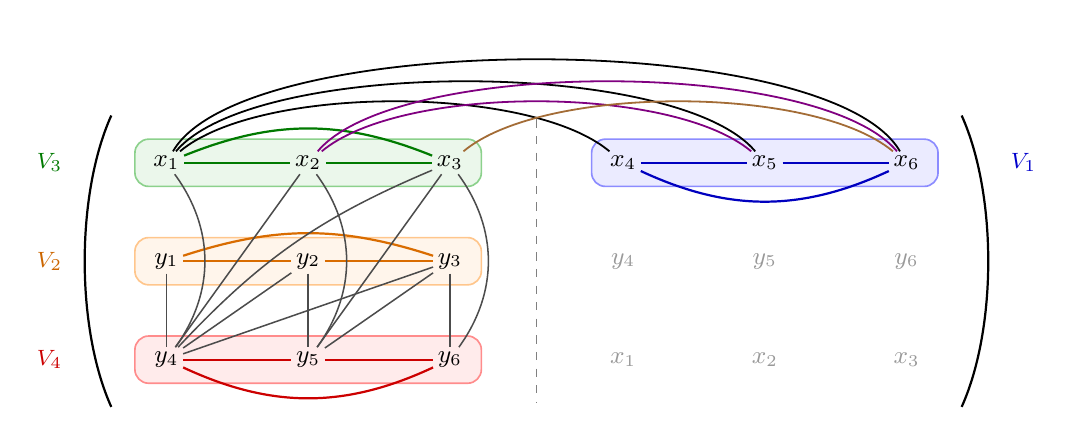
\begin{tikzpicture}[x=1cm, y=1cm,
  entry/.style={inner sep=1.5pt, font=\small},
  copy/.style={inner sep=1.5pt, font=\small, text=black!40},
  clique/.style={rounded corners=5pt, fill=#1!8, draw=#1!45, line width=0.6pt},
  cliquelab/.style={font=\footnotesize, text=#1!80!black},
  inedge/.style={line width=0.8pt, draw=#1},
  xedge/.style={line width=0.55pt, draw=black!70},
  xarc/.style={line width=0.65pt, draw=#1}
]
% Colors of the four cliques
\colorlet{Vone}{blue}
\colorlet{Vtwo}{orange}
\colorlet{Vthree}{green!60!black}
\colorlet{Vfour}{red}
 
% Cliques: V_3, V_2, V_4 in the left block, V_1 in the first row on the right
\draw[clique=Vthree] (-0.4, 0.3)  rectangle (4.0,-0.3);   % V_3
\draw[clique=Vtwo]   (-0.4,-0.95) rectangle (4.0,-1.55);  % V_2
\draw[clique=Vfour]  (-0.4,-2.2)  rectangle (4.0,-2.8);   % V_4
\draw[clique=Vone]   ( 5.4, 0.3)  rectangle (9.8,-0.3);   % V_1
 
% Separator between the two blocks
\draw[dashed, gray] (4.7,0.55) -- (4.7,-3.05);
 
% Parentheses
\draw[line width=0.8pt]
  (-0.7,0.6) .. controls (-1.15,-0.4) and (-1.15,-2.1) .. (-0.7,-3.1);
\draw[line width=0.8pt]
  (10.1,0.6) .. controls (10.55,-0.4) and (10.55,-2.1) .. (10.1,-3.1);
 
% Matrix entries: row 1 = a1..a6, row 2 = b1..b6, row 3 = c1..c6
\foreach \idx/\col/\lab in {1/0/x_1, 2/1.8/x_2, 3/3.6/x_3, 4/5.8/x_4, 5/7.6/x_5, 6/9.4/x_6}
  \node[entry] (a\idx) at (\col,0) {$\lab$};
\foreach \idx/\col/\lab in {1/0/y_1, 2/1.8/y_2, 3/3.6/y_3}
  \node[entry] (b\idx) at (\col,-1.25) {$\lab$};
\foreach \idx/\col/\lab in {1/0/y_4, 2/1.8/y_5, 3/3.6/y_6}
  \node[entry] (c\idx) at (\col,-2.5) {$\lab$};
% repeated variables (gray copies, not new vertices)
\foreach \col/\lab in {5.8/y_4, 7.6/y_5, 9.4/y_6}
  \node[copy] at (\col,-1.25) {$\lab$};
\foreach \col/\lab in {5.8/x_1, 7.6/x_2, 9.4/x_3}
  \node[copy] at (\col,-2.5) {$\lab$};
 
% Edges inside the cliques (each clique is a K_3, drawn once;
% the arc of V_1 goes below the first row to leave room for E_{13})
\draw[inedge=Vthree!80!black] (a1) -- (a2) -- (a3);
\draw[inedge=Vthree!80!black] (a1) to[bend left=22] (a3);
\draw[inedge=Vtwo!85!black]   (b1) -- (b2) -- (b3);
\draw[inedge=Vtwo!85!black]   (b1) to[bend left=18] (b3);
\draw[inedge=Vfour!80!black]  (c1) -- (c2) -- (c3);
\draw[inedge=Vfour!80!black]  (c1) to[bend right=25] (c3);
\draw[inedge=Vone!75!black]   (a4) -- (a5) -- (a6);
\draw[inedge=Vone!75!black]   (a4) to[bend right=25] (a6);
 
% E_{34}: rows 1 and 3 of the left block, region of the T_{ij}
% (the bent edges avoid the entries of the second row)
\draw[xedge] (a1) to[bend left=36]  (c1);  % x_1 y_4
\draw[xedge] (a2) --                (c1);  % x_2 y_4
\draw[xedge] (a2) to[bend left=36]  (c2);  % x_2 y_5
\draw[xedge] (a3) to[bend right=12] (c1);  % x_3 y_4
\draw[xedge] (a3) --                (c2);  % x_3 y_5
\draw[xedge] (a3) to[bend left=36]  (c3);  % x_3 y_6
 
% E_{24}: rows 2 and 3 of the left block, region of the Q_{ij}
\draw[xedge] (b1) -- (c1);  % y_1 y_4
\draw[xedge] (b2) -- (c1);  % y_2 y_4
\draw[xedge] (b2) -- (c2);  % y_2 y_5
\draw[xedge] (b3) -- (c1);  % y_3 y_4
\draw[xedge] (b3) -- (c2);  % y_3 y_5
\draw[xedge] (b3) -- (c3);  % y_3 y_6
 
% E_{13}: arcs over the first row, x_j -- x_{3+i} for j <= i,
% colored by their endpoint in V_3
\draw[xarc=black]         (a1) to[bend left=40, looseness=0.62] (a4);  % x_1 x_4
\draw[xarc=black]         (a1) to[bend left=50, looseness=0.54] (a5);  % x_1 x_5
\draw[xarc=black]         (a1) to[bend left=60, looseness=0.50] (a6);  % x_1 x_6
\draw[xarc=violet]        (a2) to[bend left=40, looseness=0.62] (a5);  % x_2 x_5
\draw[xarc=violet]        (a2) to[bend left=50, looseness=0.54] (a6);  % x_2 x_6
\draw[xarc=brown!85!black](a3) to[bend left=40, looseness=0.62] (a6);  % x_3 x_6
 
% Names of the cliques
\node[cliquelab=Vthree, anchor=east] at (-1.2, 0)    {$V_3$};
\node[cliquelab=Vtwo,   anchor=east] at (-1.2,-1.25) {$V_2$};
\node[cliquelab=Vfour,  anchor=east] at (-1.2,-2.5)  {$V_4$};
\node[cliquelab=Vone,   anchor=west] at (10.6, 0)    {$V_1$};
\end{tikzpicture}
\caption{The graph $\overline{G}$ for $q=3$.}
\label{Figure: complement graph}
\end{figure}

	Now let $\mathcal O$ be the following ordering of vertices of $\overline{G}$: 
    $$\mathcal{O}=(x_{q+1},\ldots,x_{2q},\;
		y_1,\ldots,y_q,\;
		x_1,\ldots,x_q,\;
		y_{q+1},\ldots,y_{2q}).$$ 
    We claim that $\mathcal{O}$ is a perfect elimination ordering of $\overline{G}$. 
	
	Fix $1\leq i\leq q$. From the description of the edges of $\overline{G}$ it is easy to see that:
    \begin{itemize}
        \item $
	N_{\overline{G}}^+(x_{q+i})
	=
	\{x_{q+k}:i<k\leq q\}
	\cup
	\{x_j:1\leq j\leq i\};$
    \item $N_{\overline{G}}^+(y_i)
	=
	\{y_k:i<k\leq q\}
	\cup
	\{y_{q+j}:1\leq j\leq i\};$
    \item $N_{\overline{G}}^+(x_i)
	=
	\{x_k:i<k\leq q\}
	\cup
	\{y_{q+j}:1\leq j\leq i\}$;
    \item $N_{\overline{G}}^+(y_{q+i})
	=
	\{y_{q+k}:i<k\leq q\}.$
    \end{itemize}
    The last
one is contained in $V_4$, hence it is a clique. Each of the other
three is the union of a subset of one clique and a subset of another
one (of $V_1$ and $V_3$, of $V_2$ and $V_4$, and of $V_3$ and $V_4$,
respectively), so it suffices to check that every vertex of the first
subset is adjacent to every vertex of the second. Such a pair has the
form $\{x_{q+k},x_j\}$, $\{y_k,y_{q+j}\}$ or $\{x_k,y_{q+j}\}$ with
$k>i\geq j$, and it is an edge since $k\geq j$.
Hence $\mathcal O$ is a perfect elimination ordering of
$\overline{G}$, as we claimed. 

It follows that $\overline{G}$ is chordal and, in conclusion, that $J=\operatorname{in}_{<_{\mathrm{lex}}}(I(X_{3,n}))$ has a linear resolution. This concludes the proof.
\end{proof}

%=%=%=%=%=%=%=%=%=%=%=%=%=%=%=%=%=%=%=%=%=%=%=%=%=%=%=%=%=

    \begin{Corollary}\label{cor:m3-linear}
Assume that $m=3$ and that $\mathcal G_X$ is a disjoint union of
row-distinct directed cycles of length $2$. Then $I(X_{3,n})$ has a
linear resolution.
\end{Corollary}

\begin{proof}
By Proposition~\ref{prop:m=3linres}, $\operatorname{reg}\operatorname{in}_{<_{\mathrm{lex}}}(I(X_{3,n}))=2.$ Since
\[
\operatorname{reg} I(X_{3,n})
\leq
\operatorname{reg}\operatorname{in}_{<_{\mathrm{lex}}}(I(X_{3,n})),
\]
see \cite[Theorem 3.3.4]{HHgtm260}, we have $\operatorname{reg} I(X_{3,n})\leq2$. Since
$I(X_{3,n})$ is generated by quadratic forms, it follows that $\operatorname{reg} I(X_{3,n})=2.$ Hence $I(X_{3,n})$ has a linear resolution.
\end{proof}
This completes the proof of Theorem~\ref{thm:PCML-classification}.

%=%=%=%=%=%=%=%=%=%=%=%=%=%=%=%=%=%=%=%=%=%=%=%=%=%=%=%=%=
%=%=%=%=%=%=%=%=%=%=%=%=%=%=%=%=%=%=%=%=%=%=%=%=%=%=%=%=%=

\begin{Remark}\label{rem:pcml-scrolls}
{\em
All the PCML ideals appearing in
Theorem~\ref{thm:PCML-classification}
define rational normal scrolls.
In case (i), this is the scroll
$S(3,\ldots,3)$, with $n/2$ entries,
as discussed in Section~\ref{subsec:m=3}.
In case (ii), let $y_1=x_2^{(i)}$ and
$y_2=x_1^{(k)}$ with $i\neq k$.
After a permutation of the columns,
the transpose of $X_{m,2}$ is
\[
\begin{pmatrix}
x_1^{(i)} & x_2^{(i)} & x_1^{(k)}
& x_1^{(r_1)} & \cdots & x_1^{(r_{m-3})}\\
x_2^{(i)} & x_1^{(k)} & x_2^{(k)}
& x_2^{(r_1)} & \cdots & x_2^{(r_{m-3})}
\end{pmatrix},
\]
where
$\{r_1,\ldots,r_{m-3}\}
=[m-1]\setminus\{i,k\}$.
Hence $I(X_{m,2})$ defines the scroll $S(3,1,\ldots,1)$,
with $m-3$ entries equal to $1$.
}
\end{Remark}

%=%=%=%=%=%=%=%=%=%=%=%=%=%=%=%=%=%=%=%=%=%=%=%=%=%=%=%=%=%=%=%=%=%=%=
We conclude with a general remark on the relationship
between the PCML property and normality.

\begin{Remark}
{\em 
Let $I\subseteq S=K[x_1,\ldots,x_N]$ be a homogeneous
prime ideal generated by quadratic forms such that
$S/I$ is Cohen--Macaulay and $I$ has a linear
resolution. If $K$ is algebraically closed, then
$S/I$ is normal. Indeed, $I$ defines a variety of
minimal degree, and the classical classification
of such varieties implies normality; see
\cite{EG84,EH87}.

Over an arbitrary field, however, these conditions
do not necessarily imply normality. For example,
$I=(x^2+y^2)\subseteq\mathbb{R}[x,y]$ is prime,
$S/I$ is Cohen--Macaulay, and $I$ has a linear
resolution, but $S/I$ is not normal.

On the other hand, if $I$ is a toric ideal, then
$S/I$ is an affine semigroup ring. Since a toric
ideal remains prime after extending the field
to its algebraic closure, and the normality of
an affine semigroup ring is independent of the
base field \cite[Proposition~1]{Hochster1972},
it follows that $S/I$ is normal over any field $K$.
}
\end{Remark}



\begin{thebibliography}{99}

\bibitem{BrunsConcaRaicuVarbaro}
W.~Bruns, A.~Conca, C.~Raicu and M.~Varbaro,
\emph{Determinants, Gr\"obner Bases and Cohomology},
Springer Monographs in Mathematics,
Springer, Cham, 2022.

\bibitem{BrunsHerzog}
W.~Bruns and J.~Herzog,
\emph{Cohen--Macaulay Rings},
Cambridge Studies in Advanced Mathematics, Vol.~39,
Cambridge University Press, Cambridge, 1993.

\bibitem{BrunsVetter}
W.~Bruns and U.~Vetter,
\emph{Determinantal Rings},
Lecture Notes in Mathematics, Vol.~1327,
Springer-Verlag, Berlin, 1988.

%\bibitem{B} P.~Buneman, A characterization of rigid circuit graphs, {\em Discrete Math.} {\bf 9} (1974), 205--212.

\bibitem{EisenbudSyzygies}
D.~Eisenbud,
\emph{The Geometry of Syzygies: A Second Course in Commutative Algebra and Algebraic Geometry},
Graduate Texts in Mathematics, Vol.~229,
Springer, New York, 2005.

\bibitem{EG84}
D.~Eisenbud and S.~Goto,
Linear free resolutions and minimal multiplicity,
\emph{J. Algebra} \textbf{88} (1984), 89--133.

\bibitem{EH87}
D.~Eisenbud and J.~Harris,
On varieties of minimal degree (a centennial account),
in \emph{Algebraic Geometry, Bowdoin, 1985},
Proc. Sympos. Pure Math., Vol.~46, Part~1,
Amer. Math. Soc., Providence, RI, 1987, pp.~3--13.

\bibitem{F}
R.~Fr\"oberg,
On Stanley--Reisner rings,
in \emph{Topics in Algebra, Part~2 (Warsaw, 1988)},
Banach Center Publ., Vol.~26,
PWN, Warsaw, 1990, pp.~57--70.

\bibitem{FG}
D.~R.~Fulkerson and O.~A.~Gross,
Incidence matrices and interval graphs,
\emph{Pacific J. Math.} \textbf{15} (1965), 835--855.

\bibitem{HHgtm260}
J.~Herzog and T.~Hibi,
\emph{Monomial Ideals},
Graduate Texts in Mathematics, Vol.~260,
Springer, London, 2011.

%\bibitem{Hibi} T.~Hibi, Distributive lattices, affine semigroup rings and algebras with straightening laws, {\it in} ``Commutative Algebra and Combinatorics'' (M. Nagata and H. Matsumura, Eds.), Advanced Studies in Pure Math., Volume 11, North--Holland, Amsterdam, 1987, pp. 93--109.

\bibitem{HQ}
T.~Hibi and A.~A.~Qureshi,
Prime and Cohen--Macaulay ideals of $2$-minors with linear resolution,
arXiv:2609.23712, 2026.

\bibitem{HQS}
T.~Hibi, A.~A.~Qureshi and S.~Saeedi Madani,
Prime and Cohen--Macaulay binomial ideals with linear resolution,
arXiv:2607.22127, 2026.

\bibitem{Hochster1972}
M.~Hochster,
Rings of invariants of tori, Cohen--Macaulay rings generated by monomials, and polytopes,
\emph{Ann. of Math. (2)} \textbf{96} (1972), 318--337.

\bibitem{Rose}
D.~J.~Rose,
Triangulated graphs and the elimination process,
\emph{J. Math. Anal. Appl.} \textbf{32} (1970), 597--609.

\bibitem{Stu}
B.~Sturmfels,
\emph{Gr\"obner Bases and Convex Polytopes},
University Lecture Series, Vol.~8,
Amer. Math. Soc., Providence, RI, 1996.

\end{thebibliography}


\bigskip

\begin{footnotesize}
{\bf Declaration of competing interest.}  The authors declare that they have no known competing financial interests or personal relationships that could have appeared to influence the work reported in this paper.

\medskip

{\bf Data availability.} No data was used for the research described in the article. 

\medskip

\end{footnotesize}










\end{document}
